
%%% Hlavní soubor. Zde se definují základní parametry a odkazuje se na ostatní části. %%%
% Meta-data o práci (je nutno upravit)
\input metadata.tex

% Vygenerujeme metadata ve formátu XMP pro použití balíčkem pdfx
\input xmp.tex

%% Verze pro jednostranný tisk:
% Okraje: levý 40mm, pravý 25mm, horní a dolní 25mm
% (ale pozor, LaTeX si sám přidává 1in)
\documentclass[12pt,a4paper]{report}
\setlength\textwidth{145mm}
\setlength\textheight{247mm}
\setlength\oddsidemargin{15mm}
\setlength\evensidemargin{15mm}
\setlength\topmargin{0mm}
\setlength\headsep{0mm}
\setlength\headheight{0mm}
% \openright zařídí, aby následující text začínal na pravé straně knihy
\let\openright=\clearpage

%% Pokud tiskneme oboustranně:
% \documentclass[12pt,a4paper,twoside,openright]{report}
% \setlength\textwidth{145mm}
% \setlength\textheight{247mm}
% \setlength\oddsidemargin{14.2mm}
% \setlength\evensidemargin{0mm}
% \setlength\topmargin{0mm}
% \setlength\headsep{0mm}
% \setlength\headheight{0mm}
% \let\openright=\cleardoublepage

%% Pokud práci odevzdáváme pouze elektronicky, vypadají lépe symetrické okraje
% \documentclass[12pt,a4paper]{report}
% \setlength\textwidth{145mm}
% \setlength\textheight{247mm}
% \setlength\oddsidemargin{10mm}
% \setlength\evensidemargin{10mm}
% \setlength\topmargin{0mm}
% \setlength\headsep{0mm}
% \setlength\headheight{0mm}
% \let\openright=\clearpage

%% Vytváříme PDF/A-2u
\usepackage[a-2u]{pdfx}

%% Přepneme na českou sazbu a fonty Latin Modern
\usepackage[czech]{babel}
\usepackage{lmodern}

% Pokud nepouživáme LuaTeX, je potřeba ještě nastavit kódování znaků
\usepackage{iftex}
\ifpdftex
\usepackage[utf8]{inputenc}
\usepackage[T1]{fontenc}
\usepackage{textcomp}
\fi

%%% Další užitečné balíčky (jsou součástí běžných distribucí LaTeXu)
\usepackage{amsmath}        % rozšíření pro sazbu matematiky
\usepackage{amsfonts}       % matematické fonty
\usepackage{amsthm}         % sazba vět, definic apod.
\usepackage{bm}             % tučné symboly (příkaz \bm)
\usepackage{booktabs}       % lepší vodorovné linky v tabulkách
\usepackage{caption}        % umožní definovat vlastní popisky plovoucích objektů
\usepackage{csquotes}       % uvozovky závislé na jazyku
\usepackage{dcolumn}        % vylepšené zarovnání sloupců tabulek
\usepackage{floatrow}       % umožní definovat vlastní typy plovoucích objektů
\usepackage{graphicx}       % vkládání obrázků
\usepackage{icomma}         % inteligetní čárka v matematickém módu
\usepackage{indentfirst}    % zavede odsazení 1. odstavce kapitoly
\usepackage[nopatch=item]{microtype}  % mikrotypografická rozšíření
\usepackage{paralist}       % lepší enumerate a itemize
\usepackage[nottoc]{tocbibind} % zajistí přidání seznamu literatury,
                            % obrázků a tabulek do obsahu
\usepackage{xcolor}         % barevná sazba

\usepackage{tabularx}       % tabulky

% Balíček hyperref, kterým jdou vyrábět klikací odkazy v PDF,
% ale hlavně ho používáme k uložení metadat do PDF (včetně obsahu).
% Většinu nastavítek přednastaví balíček pdfx.
\hypersetup{unicode}
\hypersetup{breaklinks=true}

% Balíčky pro sazbu informatických prací
\usepackage{algpseudocode}  % součást balíčku algorithmicx
\usepackage[Algoritmus]{algorithm}
\usepackage{fancyvrb}       % vylepšené prostředí verbatim
\usepackage{listings}       % zvýrazňování syntaxe zdrojových textů

% Cleveref může zjednodušit odkazování, ale jeho užitečnost pro češtinu
% je minimalní, protože nezvládá skloňování.
% \usepackage{cleveref}

% Formátování bibliografie (odkazů na literaturu)
% Detailní nastavení můžete upravit v souboru macros.tex.
%
% POZOR: Zvyklosti různých oborů a kateder se liší. Konzultujte se svým
% vedoucím, jaký formát citací je pro vaši práci vhodný!
%
% Základní formát podle normy ISO 690 s číslovanými odkazy
\usepackage[natbib,style=iso-numeric,sorting=none]{biblatex}
% ISO 690 s alfanumerickými odkazy (zkratky jmen autorů)
%\usepackage[natbib,style=iso-alphabetic]{biblatex}
% ISO 690 s citacemi tvaru Autor (rok)
%\usepackage[natbib,style=iso-authoryear]{biblatex}
%
% V některých oborech je běžnější obyčejný formát s číslovanými odkazy
% (sorting=none říká, že se bibliografie má řadit podle pořadí citací):
%\usepackage[natbib,style=numeric,sorting=none]{biblatex}
% Číslované odkazy, navíc se [1,2,3,4,5] komprimuje na [1-5]
%\usepackage[natbib,style=numeric-comp,sorting=none]{biblatex}
% Obyčejný formát s alfanumerickými odkazy:
%\usepackage[natbib,style=alphabetic]{biblatex}

% Z tohoto souboru se načítají položky bibliografie
\addbibresource{literatura.bib}

% Definice různých užitečných maker (viz popis uvnitř souboru)
\input macros.tex

%%% Titulní strana a různé povinné informační strany
\begin{document}
%%% Titulní strana práce a další povinné informační strany

%%% Nápisy na přední straně desek
%%% Pokud je práce ve slovenštině, desky mají být česky.

% Desky obvykle nesázíme, ale pokud je chcete přidat, změnte \iffalse na \iftrue
\iffalse

\pagestyle{empty}
\hypersetup{pageanchor=false}
\begin{center}

\large
Univerzita Karlova

\medskip

Matematicko-fyzikální fakulta

\vfill

{\huge\bf\ThesisTypeTitle}

\vfill

{\huge\bf\ThesisTitle\par}

\vfill
\vfill

\hbox to \hsize{\YearSubmitted\hfil \ThesisAuthor}

\end{center}

\newpage\openright
\setcounter{page}{1}

\fi

%%% Titulní strana práce
%%% Pokud je práce ve slovenštině, tato strana zůstává česky.

\pagestyle{empty}
\hypersetup{pageanchor=false}

\begin{center}

\centerline{\mbox{\includegraphics[width=166mm]{img/logo-cs.pdf}}}

\vspace{-8mm}
\vfill

{\bf\Large\ThesisTypeTitle}

\vfill

{\LARGE\ThesisAuthor}

\vspace{15mm}

{\LARGE\bfseries\ThesisTitle\par}

\vfill

\Department

\vfill

{
\centerline{\vbox{\halign{\hbox to 0.45\hsize{\hfil #}&\hskip 0.5em\parbox[t]{0.45\hsize}{\raggedright #}\cr
Vedoucí \ThesisTypeGenitive{} práce:&\Supervisor \cr
\ifx\ThesisType\TypeRig\else
\noalign{\vspace{2mm}}
Studijní program:&\StudyProgramme \cr
\fi
}}}}

\vfill

Praha \YearSubmitted

\end{center}

\newpage

%%% Strana s čestným prohlášením k práci
%%% Pokud je práce ve slovenštině, tato strana zůstává česky.

\openright
\hypersetup{pageanchor=true}
\vglue 0pt plus 1fill

\noindent
Prohlašuji, že jsem tuto \ThesisTypeAccusative{} práci vypracoval(a) samostatně a výhradně
s~použitím citovaných pramenů, literatury a dalších odborných zdrojů.
Beru na~vědomí, že se na moji práci vztahují práva a povinnosti vyplývající
ze zákona č. 121/2000 Sb., autorského zákona v~platném znění, zejména skutečnost,
že Univerzita Karlova má právo na~uzavření licenční smlouvy o~užití této
práce jako školního díla podle §60 odst. 1 autorského zákona.

\vspace{10mm}

\hbox{\hbox to 0.5\hsize{%
V \hbox to 6em{\dotfill} dne \hbox to 6em{\dotfill}
\hss}\hbox to 0.5\hsize{\dotfill\quad}}
\smallskip
\hbox{\hbox to 0.5\hsize{}\hbox to 0.5\hsize{\hfil Podpis autora\hfil}}

\vspace{20mm}
\newpage

%%% Poděkování

\openright

\noindent
\Dedication

\newpage

%%% Povinná informační strana práce

\openright
{\InfoPageFont

\vtop to 0.5\vsize{
\setlength\parindent{0mm}
\setlength\parskip{5mm}

Název práce:
\ThesisTitle

Autor:
\ThesisAuthor

\DeptType:
\Department

Vedoucí \ThesisTypeGenitive{} práce:
\Supervisor, \SupervisorsDepartment

Abstrakt:
\Abstract

Klíčová slova:
{\def\sep{\unskip, }\ThesisKeywords}

\vfil
}

\vtop to 0.49\vsize{
\setlength\parindent{0mm}
\setlength\parskip{5mm}

Title:
\ThesisTitleEN

Author:
\ThesisAuthor

\DeptTypeEN:
\DepartmentEN

Supervisor:
\Supervisor, \SupervisorsDepartmentEN

Abstract:
\AbstractEN

Keywords:
{\def\sep{\unskip, }\ThesisKeywordsEN}

\vfil
}

}

\newpage

%%% Další stránky budeme číslovat
\pagestyle{plain}


%%% Strana s automaticky generovaným obsahem práce

\tableofcontents

%%% Jednotlivé kapitoly práce jsou pro přehlednost uloženy v samostatných souborech
\chapter*{Úvod}
\addcontentsline{toc}{chapter}{Úvod}

V případě vážné nehody může být i několik minut rozdíl mezi stabilizováním pacienta nebo pacientem v kritickém stavu.
Z toho důvodu je velmi důležité plné pokrytí oblasti působnosti pohotovostní služby, ideálně zajištění pomoci do určitého času, nehledě na lokaci nebo aktuální vytíženosti.
Zároveň je žádoucí, aby zaměstanci a vozidla pohotovostních služeb byli využiti efektivně.
Chtěli bychom co nejméně zaměstanců, kteří budou naplánováni na určitý časový interval, aby byli připraveni a k dispozici v případě incidentu,
ale nakonec nebudou potřeba na výjezd, jelikož jsou nadbyteční a všechny incidenty byli vyřešeny kolegy.
Pro zajištění takových požadavků je nutné si velmi dobře rozmyslet plán pohotovostní služby.
Plán, který balancuje mezi co největším pokrytím a je připraven i na krajní případy a také mezí efektivním naplánováním pracovníku aby byli co nejvíce využiti.
K vymyšlení takového plánu je dobré vycházet z historických dat.
Všimnout si, v jakých lokalitách a v jakých časech se incidenty dějí a při rozhodování se na jaké sanitky v jakých časech budou
zaměstnanci naplánovaní brát tato data v úvahu.
Pohotovostní služby mají ovšem stovky sanitek se stovky zaměstnanci, a vymyslet optimální plán se může stát velmi rychle poměrně náročnou úlohou.
Přitom umět takový optimální plán najít je velmi žádoucí.

To nás vede na hlavní téma této práce, ve které se zabývám problematikou jak takový optimální plán najít a zkoumám metody,
které umí v rozumném čase najít jeden, nebo i více takových optimálních plánu.
Tyto metody zkoumám jak z hlediska kvality nalezených plánu, tak i jak rychle je metoda umí nalézt.
Dále zkoumám jak se metody chovají v různých scénářích.
Od normálního dne, kdy dle historických dat se incidenty dějí podle předpokládání, až po kritické situace, které plán maximálně vytíží.
Tyto metody mezi sebou i porovnávám, a ukáži jaké metody patří mezi ty nejlepší a které bych doporučil pro použití.

Data a statistiky potřebné pro zmíněnou analýzu získávám simulováním chodu pohotovostní služby s přiřazeným daným plánem, získaným některou z metodik.
Historické incidenty, podle kterých hledám optimální plány jsou syntenticky vytvořeny.
To stejné platí pro rozmístění stanic se sanitkami a výběrem lokace působnosti pohotovostní služby.
Avšak snažil jsem se data vytvořit tak, aby co nejlépe odráželi reálný svět.
Simulace je deterministická a při výběru sanitky pro obsluhu incidentu jsou navrženy pravidla tak, jak by se mohla sanitka vybírat v reálné situaci.




\chapter{Převedení na optimalizační úlohu}

\section{Formalizace problému}\label{kap:formalizaceProblemu}

Ústředním problémem pohotovostních služeb je umět naplánovat týmy záchranářů a záchranná vozidla na výjezdové stanice tak, aby efektivně odbavili co největší počet incidentů,
při nejnižších možných, vynaložených nákladech, v rámci jednoho dne.
Naším cílem je vymyslet metody, jak být schopný taková optimální naplánovaní nalézt.
Z toho důvodu je v první řadě potřeba si problém zformalizovat a jasně si tak vymezit, jaký konkrétní problém řešíme.

Pohotovostní služba má k dispozici \textit{týmy záchranářů} $Z = \{ z_1, z_2, \dots, z_{Z_n} \}$, \textit{záchranná vozidla} $A = \{ a_1, a_2, \dots\ a_{A_n} \}$
a \textit{výjezdové stanice} $V = \{ v_1, v_2, \dots, v_{V_n} \}$. 
Na území působnosti pohotovostní služby se nachází nemocnice $H = \{ h_1, h_2, \dots h_{H_n} \}$.
Pohotovostní služba definuje \textit{pracovní směny} týmů záchranářů $D = D_{s} \times D_{l}$, 
kde $D_{s} \in \mathbb{N}_0$ množina \textit{začátků pracovních směn} a $D_{l} \in \mathbb{N}_0$ množina \textit{délek pracovních směn}.
\textit{Pracovní směna} $d \in D$ je tak dvojice $d = (d_s, d_l)$, kde $d_{s} \in D_{s}$ značí začátek a $d_{l} \in D_{l}$ délku trvání směny.
Nechť $D_n = |D|$.

Plánem pohotovostní služby chápeme přiřazení týmů záchranářů $z \in Z$ a záchranných vozidel $a \in A$ na konkrétní výjezdové stanice $v \in V$
a přiřazení pracovní směny $d \in D$ každému týmu záchranářů $z \in Z$ v rámci jednoho dne.
Tato přiřazení popíšeme \textit{přiřazovacími funkcemi}:
\begin{definice}[Přiřazovací funkce]
  \begin{alignat*}{2}
    p_Z \colon Z &\rightarrow V \cup \{ v_{\emptyset} \} \quad && \hspace{30pt} \text{přiřazení týmů na stanice}, \\
    p_A \colon A &\rightarrow V \cup \{ v_{\emptyset} \} \quad && \hspace{30pt} \text{přiřazení vozidel na stanice}, \\ 
    p_{D} \colon Z &\rightarrow D                        \quad && \hspace{30pt} \text{přiřazení směn týmům}.
  \end{alignat*}
\end{definice}
Tým $z \in Z$ nemá přiřazenou žádnou výjezdovou stanici právě tehdy, když
$p_{Z}(z) = v_{\emptyset}$ a $p_{D}(z) = (d_s, d_l) \colon d_l = 0$.
Záchranné vozidlo $a \in A$ nemá přiřazenou žádnou výjezdovou stanici, právě tehdy, když $p_{A}(a) = a_{\emptyset}$.

Pro pohodlnost zaveďme:
\begin{align*}
  & p_D(z) = (d_s, d_l) \Rightarrow p_{D_s}(z) = d_s, \\
  & p_D(z) = (d_s, d_l) \Rightarrow p_{D_l}(z) = d_l.
\end{align*}

\textit{Plánem pohotovostní služby} budeme označovat 
čtveřici
\begin{align*}
  p = (p_Z, p_A, p_{D_{s}}, p_{D_{l}}) \in P,
\end{align*}
kde P je množina všech plánů pohotovostních služeb.
Množina $P$ obsahuje všechny plány, ale ne všechny plány jsou pro nás zajímavé.
Zajímat nás budou pouze plány, které splňují nějaké \textit{omezující podmínky}.
Pohotovostní služba definuje omezující podmínky, a to konkrétně \textit{maximální počty týmů záchranářů a záchranných vozidel povolených na jednotlivých výjezdových stanicích}.
\begin{definice}[Omezující podmínky pohotovostního plánu]
  Nechť $\mathbf{c^z}, \mathbf{c^a} \in \mathbb{N}^{V_n}$ vektory, 
  kde $i$-tou položku definujeme:
  \begin{align*}
    &\mathbf{c^z}_i \hspace{20pt} \text{maximální počet záchranných týmů na výjezdové stanici $v_i \in V$}, \\ 
    &\mathbf{c^a}_i \hspace{20pt} \text{maximální počet záchranných vozidel na výjezdové stanici $v_i \in V$},
  \end{align*}
  pro $1 \leq i \leq V_n$.
  Nechť omezující podmínky $C = \{ C_Z, C_A \}$, kde $C_Z \colon P \rightarrow \{ 0, 1 \}$, $C_A \colon P \rightarrow \{ 0, 1 \}$, definované:

  \begin{align*}
    C_Z(p) = 1 &\iff |\{ z \in Z \mid p_Z(z) = v_i \}| \leq \mathbf{c^z}_i, \hspace{20pt} \text{jinak 0}, \\
    C_A(p) = 1 &\iff |\{ a \in A \mid p_A(a) = v_i \}| \leq \mathbf{c^a}_i, \hspace{20pt} \text{jinak 0},
  \end{align*}
  $\forall i \colon 1 \leq i \leq V_n$, $p \in P$.
\end{definice}

Plán pohotovostní služby $p \in P$ splňující omezující podmínky $C$ je plán, který splňuje:
\begin{align*}
    C_Z(p) = 1 \land C_A(p) = 1.
\end{align*}
V opačném případě $p$ nesplňuje omezující podmínky $C$.
Označme $P_C$ jako \textit{množinu plánů splňujících omezující podmínky $C$}.

Pohotovostní plán pak bude v průběhu dne odbavovat \textit{incidenty}.
\textit{Incident} je trojice:
\begin{enumerate}
  \item místo nastání,
  \item čas nastání,
  \item požadováná maximální doba příjezdu záchranné jednotky.
\end{enumerate}
Budeme vždy uvažovat pouze incidenty, které se odehrávájí v rámci jednoho dne. Tuto množinu označme $I$.

Zároveň neexistují dva incidenty, které se odehrají v přesně stejný čas.
Tento předpoklad je bez újmy na obecnosti, protože kdyby bylo žádoucí, aby se dva incidenty odehráli v přesně stejný čas,
tak jednomu z nich stačí čas nastání posunout o vteřinu.

Problém, který v této práci řešíme, je nalézt \textit{optimální plán} $p_C \in P_C \subseteq P$,
tedy plán,
který bude maximalizovat počet \textit{úspěšně odbavených incidentů $s_I$} a minimalizovat \textit{celkovou cenu plánu $u(p)$}.

\section{Simulace plánu pohotovostní služby}\label{SimulaceKap}

Naším cílem je umět nalézt optimální plán pohotovostní služby.
Ten určujeme podle počtu úspěšně odbavených incidentů $s_I$ a ceny plánu $u(p)$.
Z toho důvodu jsme si formálně nadefinovali prostředky, které má pohotovostní služba k dispozici a co je plán pohotovostní služby.

V kapitole \ref{kap:optUloha2uc} definujeme cenu plánu $u(p)$ (viz definice \ref{df:cenaPlanu}).
V této kapitole navrhneme způsob, jakým zjistíme $s_I$ pohotovostního plánu $p$ na množine incidentů $I$.
Pro zjištění $s_I$ spustíme simulaci $s$ pohotovostního plánu $p$ na dané množině $I$.
Následně formálně popíšeme simulaci a jaká pravidla chodu simulace se rozhodneme použít.
Důvod použití přístupu simulace je popsán v nadcházející kapitole.

\subsection{Přístup použití simulace}\label{kap:procSimulace}

Je velmi důležité, aby počet úspěšně odbavených incidentů, které budeme uvažovat při optimalizaci, co nejvíce odpovídal počtu úspěšně odbavených incidentů,
kdyby byl plán $p$ použit v reálném světě, a v průběhu dne by se přesně děly incidenty $I$.
Přesně k takovému účelu se používají simulace.
Simulace bude napodobovat chování plánu v průběhu dne tak, jak by se plán skutečně choval v reálném světě.
Čím realističtěji bude simulace navžena, tím lépe bude počet úspěšně odbavených incidentů simulace odpovídat
počtu úspěšně odbavených incidentů v reálném světě.

Přístup použití simulace má ještě jednu podstatnou výhodu.
Různé pohotovostní služby mohou používat různé způsoby a pravidla, například pro výběr záchranného týmu či vozidla pro odbavení incidentu, který právě nastal, nebo do jaké nemocnice je incident vhodné odbavit.
Tato pravidla mohou být příliš složitá na to, aby bylo možné je výstižně zachytit jinými způsoby, jako například pouze matematickými rovnostmi a nerovnostmi, jak je zvykem pro lineární programování \cite{LP}.

Na druhou stranu je podstatnou nevýhodou simulace její výpočetní náročnost a značné omezení použitelných technik obecně využívaných pro řešení optimalizač~ních problémů.

\subsection{Popis deterministické diskrétní simulace}

\textit{Simulace} je proces navrhnutí modelu reálného systému, a provádění tak na něm experimenty za účelem buď porozumění chování systému
nebo vyhodnocení různých strategií chování systému.
\textit{Systém simulace} je chápan jako dobře definovaná kolekce objektů a interakcí mezi nimi.
Simulace si udržuje \textit{stav systému}. Ten definuje jak se má simulace chovat.
Systém simulace se může měnit průběhem simulace nebo při nastání \textit{události}.

Simulace obecně dělíme na \textit{spojité} a \textit{diskrétní}.
Ve \textit{spojité simulaci} se změny systému dějí kontinuálně v průběhu běhu simulace, nejčastěji podle soustavy diferenciálních rovnic.
V \textit{diskrétní simulaci} se změny sytému dějí v diskrétních časoých úsecích, nejčastěji v čase nastání nějaké \textit{události}.

Typický způsob, jakým diskrétní simulace probíhá je následovný.
Simulace odbavuje údalosti v pořadí dle času nastání.
Při inicializaci si naplánuje nějaké údalosti.
Při odbavování události aktualizuje stav systému podle jeho předchozího stavu a aktuálně odbavované události. Zároveň si simulace náplanuje další události. 
Simulace skončí jakmile nejsou žádné další události k odbavení.

Dále dělíme simulace na \textit{deterministcké} a \textit{stochastické}.
V \textit{deterministické simulaci} jsme schopni z aktuálního stavu systému a údalosti deterministicky určit nadcházející stav systému.
V \textit{stochastické simulaci} nejsme schopni z aktuálního stavu systému a údalosti deterministicky určit nadcházející stav systému.
Většinou proto, že při výběru nadhcázejícího stavu figuruje element náhody
\cite{SimulaceBook}.

\subsection{Popis deterministické diskrétní simulace plánu pohotovostní služby}\label{kap:definiceSimulace}

Abychom mohli simulovat fungování pohotovostního plánu,
potřebujeme si v první řadě definovat, jaké podmínky musí záchranný tým splňovat, aby mohl \textit{úspěšně odbavit incident}.

\begin{definice}\label{df:simulacePravidla1}
  Tým záchranářů $z \in Z$ je schopen úspěšně odbavit incident $i \in I$ právě tehdy, když:
  \begin{enumerate}
    \item
      Je alokován a má přiřazenou směnu. Pokud tým záchranářu není alokován, tj. $p_Z(z) = v_{\emptyset}$, tak samozřejmě není schopen obsloužit $i$.

    \item
      Tým je schopen dorazit na místo incidentu do \emph{požadované doby}.
      Ať už přímo z výjezdové stanice, nebo při vrácení se po vyřízení incidentu zpět na výjezdovou stanici. 
      V prvním případě tým potřebuje mít na výjezdové stanici k dispozi volné záchranné vozidlo.

    \item
      Týmu nekončí směna dříve, než je očekávaný konec celkové doby vyřízení incidentu.
  \end{enumerate}
\end{definice}

Nechť $Z_i \subseteq Z$ množina záchranných týmu, které jsou schopny úspěšně odbavit incident $i \in I$.
Pro odbavení $i$ musíme vybrat nějaký konkrétní $z_i \in Z_i$.

Je mnoho různých způsobu, jak $z_i$ vybrat.
V naší simulaci jsou použitá pravidla vybraná na základě konzultace se společností, která se danou problematikou zabývá přes 25 let
a sama podobná pravidla používá pro plánovaní u několika jejích klientů ve Spojených státech amerických \footnote{Logis Solutions, s.r.o. (https://logissolutions.net)}.

Simulace je navržena dostatečně genericky tak, aby bylo možné naimplementovat i libovolná jiná pravidla, například jednodušší, komplikovanější nebo klidně i stochastická.
Jak bylo zmíněno v kapitole \ref{kap:procSimulace}, možnost volby libovolných pravidel je jedna z více výhod přístupu použití simulace.
\begin{definice}\label{df:simulacePravidla2}
  Nejvhodnější tým záchranářů $z_i \in Z_i$, kde $Z_i \subseteq Z$ jsou všechny týmy záchranářů schopny úspěšně odbavit incident $i \in I$ je tým,
  který je nejlepší podle následujících kritérií v daném pořadí:
  \begin{enumerate}
    \item Upřednostni tým, který je na výjezdové stanici před týmem, který ještě ukončuje vyřízení jednoho z předchozích incidentů. 
    \item Upřednostni tým, který na místo incidentu dorazí dříve. 
    \item Upřednostni tým, který obsloužil méně incidentů a je tedy méně vyčerpaný.
  \end{enumerate}
\end{definice}
Pravidla výběru \textit{nejvhodnějšího týmu záchranářů} jsou navrhnuta tak,
aby práce obsluhování incidentů byla rozmístěna rovnoměrně přes všechny týmy, ale zároveň aby byly incidenty obslouženy nejrychlejším možným způsobem.

Pravidla také počítají s možným zpožděním a raději upřednostní tým, který je aktuálně k dispozici, než tým, který ještě dokončuje jiný incident,
ale mohl by být i na místě incidentu o něco dříve, pokud by neměl zpoždění. Příkladem je první pravidlo pro výběr nejvhodnějšího týmu.

Jakmile je $z_i$ vybrán, naplánujeme mu incident $i$ a $z_i$ \textit{odbavuje incident $i$}.

\clearpage

\begin{definice}[Záchranný tým odbavuje incident]\label{df:odbavujeIncident}
  Řekneme, že záchranný tým odbavuje incident, pokud vykonává následující činnosti:
  \begin{enumerate}
    \item
      Tým přijíží na místo odehrání incidentu.

    \item
      Tým odbavuje incident na místě odehrání incidentu.

    \item
      Tým pacienty z incidentu převáží do nejbližší nemocnice.

    \item
      Tým pacienty odbavuje v nemocnici.

    \item
      Tým přijíždí zpět na výjezdovou stanici.
  \end{enumerate}
\end{definice}
Definujme si funkce, které budou v simulaci používány a pomocí výše uvedených pravidel naleznou nejvhodnější tým záchranářů $z_i$
a pro něj nejvhodnější záchranné vozidlo.
\begin{definice}[GetBestTeam]\label{df:getBestTeam}
Funkce \textit{GetBestTeam} vrací tým záchranářu $z_i$ z týmů záchranářů $Z_i$, kteří jsou schopni úspěšně odbavit aktuální incident $i \in I$~(viz definice \ref{df:simulacePravidla1})
  , kde $z_i$ je nejvhodnější tým pro obsloužení incidentu $i$ ze $Z_i$~(viz definice \ref{df:simulacePravidla2}). 
\end{definice}
\begin{definice}[GetBestAmbulance]
Funkce \textit{GetBestAmbulance}\label{df:getBestAmbulance} vybere záchranné vozidlo, které je na stejné výjezdové stanici jako $z_i$ a z hlediska času je nejdříve k dispozici.
\end{definice}

Nyní jsme připraveni definovat \textit{simulaci pohotovostního plánu} $p \in P_C$ na množině incidentů $I$, a to jako deterministickou diskrétní simulaci $s$:
\begin{align*}
  s_I = s(p, I).
\end{align*}
Simulace $s$ vrátí počet úspěšně odbavených incidentů $s_I$ na množině $I$ plánem $p$. 

\textit{Událost} je nastání incidentu 
\begin{align*}
  i \in I \text{ v čase } T_I(i),
\end{align*}
kde $T_I \colon I \rightarrow \mathbb{N}_0$, určuje čas nastání incidentu.
\textit{Stav systému} simulace $s$ je množina
\begin{align*}
S = \{ S_A, S_Z \},
\end{align*}
kde $S_A$ je stav záchranných vozidel $A$ a $S_Z$ je stav týmů záchranářů $Z$. 
Stav $S_A$ je rozmístění záchranných vozidel v prostoru.
Stav $S_Z$ je informace, kdy bude záchranný tým k dispozici a pokud tým odbavuje nějaký incident, tak v jaké fázi odbavování zrovna je. 

\begin{algorithm}[H]
  \begin{algorithmic}[1]
  \Function{Simulation}{$p, I$ \mbox{setřízené podle času nastání $T_I$}}
    \State $s_I \gets 0$
    \State $T$ \gets 0
    \State $S_Z \gets \mbox{Inicializuje podle $p$}$
    \State $S_A \gets \mbox{Inicializuje podle $p$}$
    \For{$i_k \in I,~ k \in \{1, 2, \dots , |I|\}$}
      \State $T \gets \mbox{Čas nastání $i_k$, $T_I(i_k)$}$
      \State $z_k \gets \mbox{GetBestTeam($i_k, S_Z, S_A, T$)}$
      \If{$z_k \neq \emptyset$}
        \State $s_I \gets s_I + 1$
        \State $a_k \gets \mbox{GetBestAmbulance($z_k, T$)}$
        \State Plan($S_Z, z_k, i_k$)
        \State UpdateWhenFree($S_A, z_k, i_k, a_k$)
      \EndIf
    \EndFor
    \State \Return $s_I$
  \EndFunction
  \end{algorithmic}
  \caption{Simulace plánu pohotovostní služby $p$ na množině incidentů $I$}
  \label{simulaceAlgo}
\end{algorithm}

\vspace*{10px}

Průběh simulace je následovný. 
V krocích 2 až 5 simulace (viz algoritmus \ref{simulaceAlgo}) položí $s_I$ a $T$ rovno nule
a incicializuje si stavy $S_A$ a $S_Z$ podle plánu $p$.

V krocích 6 až 15 odbavuje události, takže se pohybuje po krocích v časech nastání incidentů od nejdřívějšího po nejpozdější.
V každém kroku simulace $k \in \{ 1, 2, \dots , |I|\}$ se simulace prvně pokusí deterministicky nalézt nejvhodnější $z_k \in Z$, který obslouží $i_k$,
pomocí funkce $\textit{GetBestTeam}$ (viz definice \ref{df:getBestTeam}), v kroku 8.
Pokud takový $z_k$ neexistuje, tak pokračuje v odbavování dalších incidentů.

Pokud existuje, v krocích 7 až 12 zvýší počet odbavených incidentů $s_I$ o jedna,
deterministicky nalezne pro $z_k$ nejvhodnější $a_k$, pomocí funkce \textit{GetBestAmbulance} (viz definice \ref{df:getBestAmbulance}) a
aktuální incident $i_k$ naplánuje na $z_k$ spolu s $a_k$ funkcí \textit{Plan}.
Záchranný tým $z_k$ tak \textit{odbavuje} incident $i_k$ (viz definice \ref{df:odbavujeIncident}), a čas, kdy bude opět tým $z_k$ k dispozici je nastaven na čas, kdy incident úspěšně odbaví. 
Tím se aktualizuje stav záchranných týmů $S_Z$.

V kroku 13 je funkcí \textit{UpdateWhenFree} aktualizován stav záchranných vozidel $S_A$.
konkrétně vozidlu $a_k$ se přiřadí čas, kdy bude opět k dispozici, tedy kdy má $z_k$ přijet zpět na výjezdovou stanici.

Simulace doběhne jakmile nejsou žádné další události k odbavení, respektive jakmile projde všechny incidenty, to je po $|I|$ krocích.
Simulace vrátí $s_I$, počet úspěšně odbavených incidentů.

\section{Převedení problému na optimalizační úlohu s více účelovými funkcemi}\label{kap:optUloha2uc}

V této kapitole si ukážeme, jak konkrétně budeme modelovat optimalizační úlohu nalezení optimálního pohotovostního plánu na množině incidentů $I$,
pomocí počtu úspěšně odbavených incidentů $s_I$ a ceny plánu $u(p)$.
Dále si nadefinujeme potřebné pojmy, jako \textit{optimalizační úlohu s více nebo s jednou účelovou funkcí}.
Ukážeme si, že problém nalezení optimálního plánu je vhodné modelovat jako optimalizační úlohu s více účelovými funkcemi,
protože chceme maximalizovat počet úspěšně odbavených incidentů a zároveň minimalizovat cenu plánu.

\begin{definice}[Optimalizační úloha s jednou účelovou funkcí \cite{AlgOptBook}]\label{df:optUloha1ucObecne}
  Optimalizační úloha s jednou účelovou funkcí je definována jako úloha nalezení $x^*$,
  \begin{align}
    x^* = \max_{x \in \mathcal{X}} \{ q(x) \},
  \end{align}
  kde $\mathcal{X}$ je množina všech možných konfigurací a $q \colon \mathcal{X} \rightarrow \mathbb{R}$ je účelová funkce.
\end{definice}

Návrh účelové funkce zásadně ovlivní, jaké $x$ je řešením.
Bez újmy na obecnosti můžeme účelovou funkci maximalizovat, protože
\begin{align*}
  \min_{x \in \mathcal{X}} \{ q(x) \} \equiv \max_{x \in \mathcal{X}} - \{ q(x) \}.
\end{align*}

Za \textit{optimální řešení optimalizační úlohy s jednou účelovou funkcí} se považuje optimální konfigurace $x^* \in \mathcal{X}$,
kde $q(x^*)$ je globální maximum $q$.
Optimální řešení nemusí být jenom jedno, může jich být více. Zároveň alespoň jedno optimální řešení vždy existuje.

\begin{definice}[Optimalizační úloha s více účelovými funkcemi]\label{df:optUloha2ucObecne}
  Optimalizační úloha s více účelovými funkcemi je definována jako úloha nalezení $x^*$,
  \begin{align*}
    x^* = \max_{x \in \mathcal{X}} \{ \mathbf{q}(x) \}, \hspace{50pt} &\mathbf{q}(x) = [q_1(x), q_2(x), \dots q_{m}(x)], q_i \in \mathcal{Q},
  \end{align*}
  pro $1 \leq i \leq m, m = |\mathcal{Q}|$,
  kde $\mathcal{X}$ je množina všech možných konfigurací a $\mathcal{Q}$ je množina všech účelových funkcí, které chceme maximalizovat.
  Víceúčelovou funkci $\mathbf{q}(x)$ maximalizujeme po složkách.
\end{definice}
Z definice \ref{df:optUloha2ucObecne} je \textit{optimálním řešením optimalizační úlohy s více účelovými funkcemi}
$x^* \in \mathcal{X}$ takzvaný \textit{utopia point} $y^{utopia}$ \cite{AlgOptBook}.
To je konfigurace, která nabývá optima pro každou jednotlivou účelovou funkci.
Zřejmě $y^{utopia}$ nemusí existovat, protože často maximalizování $q_i \in \mathcal{Q}$ může minimalizovat $q_j \in \mathcal{Q}, i \neq j$.
V nadcházející kapitole si ukážeme jak se optimalizace takového typu řeší.

V předchozí kapitole jsme si ukázali způsob, jakým nalezneme počet úspěšně odbavených incidentů $s$. 
Abychom mohli problém nalezení optimálního plánu modelovat jako optimalizační úlohu s více účelovými funkcemi, potřebujeme si ještě dodefinovat cenu plánu.
\begin{definice}[Cena plánu $u$]\label{df:cenaPlanu}
  Cena plánu $u \colon P \rightarrow \mathbb{N}$,
  \begin{align*}
    u(p) = \sum_{z \in Z} p_{D_l}(z) + |\{ a \in A \mid p_{A}(a) \neq v_{\emptyset} \}|.
  \end{align*}
  Cena plánu je součet všech dob trvání směn přiřazených záchranným týmům a počtu naalokovaných záchranných vozidel.
\end{definice}

Všimněme si, že $p_{D_l}(z) = 0$, pro nenaalokované týmy (viz kapitola \ref{kap:formalizaceProblemu}), čili nijak nepřispějí do výsledku sumy.

Nyní již máme všechny prostředky potřebné k tomu, abychom modelovali problém nalezení optimálního plánu jako optimalizační úlohu s více účelovýmí funkcemi. 
\begin{definice}[Nalezení optimálního plánu pohotovostní služby jako optimalizační úloha s více účelovými funkcemi]\label{df:optUloha2uc}
  Nalezení optimálního plánu pohotovostní služby jako optimalizační úloha s více účelovými funkcemi je úloha nalezení $p^*$,
  \begin{align*}
    p^* = \max_{p \in P_C} \{ \mathbf{q}(p) \}, \hspace{50pt} \mathbf{q}(p) = [s(p, I), -u(p)],
  \end{align*}

  kde $P_C$ je množina všech povolených plánu pohotovostní služby splňující omezení $C$ a $I$ je daná množina incidentů.
  Účelové funkce $s$ a $u$ jsou simulace plánu $p$ na $I$ a cena plánu $p$.
\end{definice}

Všimněmě si, že maximalizování $s$ bude velmi pravděpodobně vést k maximalizování $u$, tedy k minimalizování $-u$.
Plány úspěšně odbavující incidenty zřejmě budou používát více záchranných týmu s delšími směnami a více záchranných vozidel, takže budou dražší.
Z toho důvodu řešení $y^{utopia}$ nemusí existovat. Tímto problémem se zabýváme v následující kapitole.

\section{Metody pro řešení optimalizačního problému s více účelovými funkcemi}\label{kap:metodyProReseniOptSViceUcel}

V předchozí kapitole jsme problém nalezení optimálního plánu pohotovostní služby namodelovali jako optimalizační úlohu s více účelovými funkcemi (viz definice \ref{df:optUloha2uc}),
a to počtem úspěšně odbavených incidentů $s(p, I)$ a ceny plánu $u(p)$.
Zároveň jsme pozorovali, že maximalizováním $s$ minimalizujeme $-u$ a naopak.

Optimalizační úlohy s více účelovými funkcemi, mezi kterými je potřeba nalézt kompromis pro nalezení optima, jsou velmi časté,
a proto existuje několik metod, které optimalizační úlohy s více účelovými funkcemi řeší.
Jednou z účinných metod je převod víceúčelové funkce na jednu účelovou funkci, aby
zároveň maximalizování víceúčelové funkce bylo stejné jako maximalizování jedné účelové funkce.

Řešení optimalizační úlohy s jednou účelovou funkcí je dobře definované,
narozdíl od řešení optimalizační úlohy s více účelovými funkcemi.
V této kapitole si ukážeme vybrané metody.

\subsection{Lexikografické porovnání}

Jedná se o způsob převedení víceúčelové funkce pouze na jednu účelovou funkci, kde konfigurace porovnáváme lexikograficky podle permutace jednotlivých účelových funkcí,
která určuje jejich prioritu nad ostatními.

\begin{definice}[lexikografické porovnání]\label{df:lexPorovnani}
  Účelová funkce $q$ porovnávájící $x_1, x_2 \in \mathcal{X}$ lexikograficky podle permutace $\pi \in S_m$ je definovaná:
  \begin{align*}
    q(x_1) < q(x_2) \Leftrightarrow \bigvee_{k=1}^m \left ( \left ( \bigwedge_{i=1}^{k-1} q_{\pi(i)}(x_1) = q_{\pi(i)}(x_2) \right ) \land q_{\pi(k)}(x_1) < q_{\pi(k)}(x_2) \right )
  \end{align*}
  a 
  \begin{align*}
    q(x_1) = q(x_2) \Leftrightarrow q_{\pi(i)}(x_1) = q_{\pi(i)}(x_2), \forall i \in \{ 1, \dots, m \}.
  \end{align*}
\end{definice}

Jedná se o optimalizaci po jednotlivých účelových funkcích podle určené priority. 
Obecně není vhodná, protože neumí nalézt kompromis mezi jednotlivými účelovými funkcemi a často nemusí být jasné, jaké účelové funkce chceme preferovat.

\subsection{Vážená suma účelových funkcí}\label{kap:vazenaSumaUcelF}

Jedná se o způsob převedení víceúčelové funkce pouze na jednu účelovou funkci pomocí sumy účelových funkcí pronásobené jejich přidělenými váhami.

\begin{definice}[Vážená suma účelových funkcí \cite{AlgOptBook}]\label{df:vazenaSumaUcelF}
  Vážená suma účelových funkcí $q'$ je definovaná jako
  \begin{align*}
    q'(x) = w^T \mathbf{q}(x),
  \end{align*}
  kde $w \in \mathbb{R}^m$ je vektor vah.
\end{definice}

Tato metoda už umí nalézt kompromis mezi jednotlivými účelovými funkcemi, a to podle vah $w$.
Stejně ale jako u lexikografického porovnání nemusí být obecně jasné, jaké účelové funkce preferovat.

\subsection{Goal programming}\label{kap:goalP}

Jedná se o způsob převedení víceúčelové funkce pouze na jednu účelovou funkci minimalizováním vzdálenosti od nějaké ideální hodnoty -- cíle. 

\begin{definice}[Účelová funkce měřící vzdálenost od cíle \cite{AlgOptBook}]\label{df:goalP}
  \begin{align*}
    \min_{x \in \mathcal{X}} \{ \| \mathbf{q}(x) - y^{goal} \| \}, \hspace{50pt} y^{goal} \in \mathbb{R}.
  \end{align*}
\end{definice}

Standardně $y^{goal} = \mathbf{q}(y^{utopia})$.
Zvolením vhodné normy můžeme preferovat námi vybrané účelové funkce, ale obdodně jako u předchozích metod, obecně nemusí být jasné, jaké účelové funkce preferovat.
Zvolením normy jako nějaké $p$-normy (například standardní euklidovské normy), budou účelové funkce implicitně preferovány podle toho,
v jakých jednotkách se měří. Tudiž při maximalizaci budou preferovány účelové funkce s oborem hodnot ve větším rozsahu.

\subsection{Vážená exponenciální suma účelových funkcí}\label{kap:vazenaSumUcF}

Jedná se o kombinaci metody goal programming a metody vážené sumy účelových funkcí.
Váhami $w$ jsme schopni určit, kterou účelovou funkci je pro nás důležitější optimalizovat a parametrem $\varphi$ jakou $\varphi$-normu chceme použít.

\begin{definice}[Vážená exponenciální suma účelových funkcí \cite{AlgOptBook}]\label{df:vazenaSumUcF}
  \begin{align*}
    q(x) = \sum_{i=1}^{m} w_i (q_i(x) - y_i^{goal})^\varphi,
  \end{align*}
  kde $w \in \mathbb{R}^m, \varphi \in \mathbb{R}$.
\end{definice}

Může být příjemnější na použití než goal programming, protože místo škálování prostoru normou škálujeme pomocí jednotlivých hodnot účelové funkce.

\section{Převedení problému na optimalizační úlohu s jednou účelovou funkcí}\label{kap:opt1Uc}

Nadefinovali jsme účelové funkce $s$ a $u$ a problém nalezení optimálního plánu jako optimalizační úlohu s více účelovými funkcemi $s$ a $u$.
Pro optimalizační úlohy s více účelovými funkcemi obecně nemusí existovat optimum.
Proto jsme si v předchozí kapitole ukázali několik přístupů,
které vhodně převedou optimalizační úlohu s více účelovými funkcemi na optimalizační úlohu s jednou účelovou funkcí.

V této kapitole si ukážeme, jak optimalizační úlohu nalezení optimálního plánu pohotovostní služby s více účelovými funkcemi (viz definice \ref{df:optUloha2uc}) převést na
optimalizační úlohu nalezení optimálního plánu pohotovostní služby s jednou účelovou funkcí, pomocí metod zmíněných v předchozí kapitole.

K tomu si je ještě potřeba první dodefinovat přeškálované účelové funkce do intervalu $\langle 0, 1 \rangle$, aby
bylo možné výsledné účelové funkce definovat přehledněji.
\begin{definice}[Přeškálování $s$ do intervalu $\langle 0, 1 \rangle$ ] \label{df:simulaceSkal}
  Definujme $s'$ jako přeškálování $s$ do intervalu $\langle 0, 1 \rangle$,
  \begin{align*}
    s'(p, I) = s(p, I) / |I|.
  \end{align*}
\end{definice}
\begin{definice}[Přeškálování $u$ do intervalu $\langle 0, 1 \rangle$ ] \label{df:cenaPlanuSkal}
  Definujme $u'$ jako přeškálování $u$ do intervalu $\langle 0, 1 \rangle$,
  \begin{align*}
    u'(p) = u(p) / K,
  \end{align*}
  kde $K$ je maximální možná cena plánu,
  \begin{align*}
    K = Z_n \cdot \max_{d_l} \{ d_s \} + A_n,
  \end{align*}
  naalokování nejdelší směny na všechny týmy záchranářů a naalokování všech záchranných vozidel.
\end{definice}

Nyní už si můžeme ukázat jak vypadají jednotlivé účelové funkce optimalizace pohotovostního plánu.
Začneme aplikováním lexikografického porovnání (viz definice \ref{df:lexPorovnaniPohotovost}) na náš problém, a to následovně:
\begin{definice}[Lexikografické porovnávání optimalizace pohotovostního plánu]\label{df:lexPorovnaniPohotovost}
  Lexikografické porovnávání optimalizace pohotovostního plánu $q^{\text{Lex}}$ definujeme jako
  \begin{align*}
    & q^{\text{Lex}}(p_1) < q^{\text{Lex}}(p_2)\Leftrightarrow\\
    & ( s(p_1, I) < s(p_2, I)) \lor (s(p_1, I) = s(p_2, I) \land u(p_1) < u(p_2))
  \end{align*}
  a 
  \begin{align*}
    q^{\text{Lex}}(p_1) = q^{\text{Lex}}(p_2) \Leftrightarrow s(p_1, I) = s(p_2, I) \land u(p_1) = u(p_2),
  \end{align*}
  pro danou množinu incidentů $I$.
\end{definice}

Pokud za účelovou funkci zvolíme $q^{\text{Lex}}$, tak optimální plán bude takový, že odbaví co nejvíce incidentů je možné, a z nich budou optimální ty nejlevnější plány:
\begin{alignat*}{2}
  \min_{p^* \in P} \{ u(p^*) \}, && \hspace{15pt} P = \{ p \mid \max_{p \in P_C} \{ s(p, I) \} \},
\end{alignat*}
pro danou množinu incidentů $I$.

Definovat $q^{\text{Lex}}$ obráceně nedává smysl, protože nejlevnější plán je prázdný plán a ten na množině incidentů $I$ nikdy neodbaví žádný incident.

Váženou sumu účelových funkcí (viz definice \ref{df:vazenaSumaUcelF}) aplikujeme na náš problém podle následující definice. 
\begin{definice}[Vážená suma účelových funkcí optimalizace pohotovostního plánu]\label{df:vazenaSumaPohotovost}
  Váženou sumu účelových funkcí optimalizace pohotovostního plánu $q_{\alpha}$ definujeme jako
  \begin{align*}
    q_{\alpha}(p) = \alpha \cdot s'(p, I) - (1 - \alpha) \cdot u'(p), \hspace{50pt} \alpha \in [0, 1], p \in P_C,
  \end{align*}
  pro danou množinu incidentů $I$, kde $w_1 = \alpha$ a $w_2 = 1 - \alpha$.
\end{definice}

Parametr $\alpha$ bychom preferovali blíže jedné, pro upřednostnění $s'$ a pro upřednostnění $u'$ blíže nule.

Metodu goal programming (viz definice \ref{df:goalP}) aplikujeme následovně.
\begin{definice}[Goal programming optimalizace pohotovostního plánu]
  Víceúčelovou funkci převedeme na jednu podle metody goal programming na účelovou funkci $q^{\text{Goal}}$ definovanou jako
  \begin{align*}
    q^{Goal}(p) = \| [1 - s'(p, I), u'(p)] \|,
  \end{align*}
  pro danou množinu incidentů $I$ a libovolnou normu.
\end{definice}

Pro pohotovostní plány nechť $p^{goal} \colon q(p^{utopia}) = [1, 0]$, úspěšné odbavení všech incidentů za nulovou cenu.
Samozřejmě $p^{utopia} \not \in P_C$, ledaže $|I| = 0$.

Nulovou cenu má pouze plán, kde není naalokován žádný tým záchranářů ani záchranné vozidlo a takový plán nemůže úspěšně obsloužit žádný incident. 
Můžeme však měřit, jak blízko $q(p)$ k $q(p^{utopia})$ je.

Jako poslední aplikujeme na náš problém metodu vážené exponenciální sumy účelových funkcí (viz definice \ref{df:vazenaSumUcF}).
\begin{definice}[Vážená exponenciální suma účelových funkcí optimalizace pohotovostního plánů]\label{df:vazenaSumaExpPohotovost}
  Váženou exponenciální sumou účelových funkcí optimalizace pohotovostního plánů $q_{\alpha}^{\varphi}$ definujeme jako 
  \begin{align*}
    q_{\alpha}^{\varphi}(p) = \alpha (1 - s'(p, I))^\varphi + (1 - \alpha)(u'(p))^\varphi, \hspace{50pt} p \in P_C,
  \end{align*}
  pro danou množinu incidentů $I$, kde $w_1 = \alpha$ a $w_2 = 1 - \alpha$.
\end{definice}

Stejně jako u vážené sumy účelových funkcí jsme díky parametru $\alpha$ schopni upřednostit maximalizování $s'$ nad $-u'$.

Nyní máme prostředky pro definování problému nalezení optimálního pohotovostního plánu jako optimalizační úlohy s jednou účelovou funkcí.

Označme si $Q_I = \{ q^{\text{Lex}}, q^{\text{Goal}}, q_{\alpha}, q_{\alpha}^{\varphi}\}$ jako množinu účelových funkcí na dané množině incidentů $I$.
\begin{definice}[Problém nalezení optimálního plánu jako optimalizační úloha s jednou účelovou funkcí]\label{df:optUloha1uc}
  Optimalizační úloha nalezení optimálního plánu pohotovostní služby s jednou účelovou funkcí je definována jako úloha nalezení $p^*$,
  \begin{align}
    p^* = \max_{p \in P_C} \{ q(p) \},
  \end{align}
  kde $q \in Q_I$.
\end{definice}

\section{Analýza optimalizační úlohy}

V předchozí kapitole se nám podařilo problém nalezení optimálního plánu namodelovat jako optimalizační úlohu s jednou účelovou funkcí,
pomocí metod diskutovaných v kapitole \ref{kap:metodyProReseniOptSViceUcel}.
V této kapitole klasifikujeme, o jakou optimalizační úlohu se jedná, a to zkoumáním účelové funkce a množiny plánů.
Zklasifikováním optimalizační úlohy budeme moct použít metodiky, které se standardně pro řešení takových úloh využívají. 
Podrobněji jsou diskutovány v kapitole \ref{chap:reseniOptUloh}.

\subsection{Analýza množiny plánů pohotovostních služeb}\label{kap:analP}

Znát velikost množiny plánů pohotovostních služeb $P$ a $P_C$ je klíčové pro navrhování metod pro nalezení optima, proto je v této kapitole spočítáme.
To platí zejména pro $P_C$, jelikož námi hledané optimum právě $P_C$ náleží.
Jaké implikace má velikost $P_C$ na zvolené metody řešení je popsáno v kapitole \ref{kap:NP}.

\begin{veta}[Velikost množiny plánů pohotovostních služeb]\label{veta:velikostP}
  Velikost plánu pohotovostní služby $P$ je rovna:
  \begin{align*}
    \sum_{i = 0}^{Z_n} {D_n}^{\binom{Z_n - i + V_n - 1}{V_n - 1}} \cdot \sum_{i = 0}^{A_n} {\binom{A_n - i + V_n - 1}{V_n - 1}}.
  \end{align*}
\end{veta}

\begin{dukaz}
  Všimněme si, že počet uspořádaných $V_n$-tic nezáporných celých čísel posčítajících se na $k$
  přičemž záleží na pořadí sčítanců, přesně odpovídá počtu naalokování záchranných týmů na výjezdové stanice, kde chceme naalokovat přesně $k$ týmů.
  Například pro $k = 10$ a $V_n = 4$ by

  \begin{align*}
    3 + 0 + 5 + 2 = 10
  \end{align*}

  odpovídalo naalokování 3 týmů na první stanici, 0 na druhou, 5 na třetí a dva na čtvrtou.
  Podle lemma o počtu uspořádaných $r$-tic nezáporných celých čísel, které se posčítají na $m$, přičemž záleží na pořadí~(\citet{Diskretka}, (2.3), str. 61),
  víme, že takových uspořádaných $V_n$-tic je

  \begin{align}
    \binom{k + V_n - 1}{V_n - 1}.
  \end{align}

  Přesčítáním přes všechny $k \in \{ 0, \dots, Z_n \}$ tak spočítáme sumu všech naalokování přes $k$ týmů záchranářů, které jsou navzájem disjunktní, takže žádnou alokaci týmů nesčítáme vícekrát.
  Každému týmu záchranářů v rámci alokace je ještě přiřazena pracovní směna, těch je $D_n$, proto $D_n$ umocňujeme. 

  Pro alokování záchranných týmů postupujeme analogicky, akorát nepřiřazujeme pracovní směny.
\end{dukaz}

\begin{veta}[Velikost množiny plánů pohotovostních služeb splňující omezení $C$]
  Velikost plánu pohotovostní služby $P_C$ splňující omezení $C$ je rovna:
  \begin{align*}
    \sum_{i=0}^{Z^c_n}{{D_n}^{\binom{Z^c_n - i + V_n - 1}{V_n - 1}}} \cdot \sum_{i = 0}^{A^c_n}\binom{A^c_n - i + V_n - 1}{V_n - 1},
  \end{align*}

  kde
  \begin{align*}
    Z^c_n = \sum_{i=1}^{V_n} c_{z_{i}}, A^c_n = \sum_{i=1}^{V_n} a_{z_{i}}.
  \end{align*}
\end{veta}

\begin{dukaz}
  Stejný jako v předchozí větě, avšak na místo, abychom vybírali ze všech záchranných týmu a vozidel,
  vybíráme ze součtu přes korespondující dostupné kapacity na výjezdových stanicích $Z^c_n$ a $A^c_n$.
\end{dukaz}

\begin{veta}[Asymptotický odhad velikosti množiny plánů pohotovostních služeb]\label{veta:asymptotP}
  Nechť $P$ množina plánu pohotovostních služeb. Pak 

  \begin{align*}
    |P| \in \mathcal{O} \left ({D_n}^{2^{Z_n + V_n}} \cdot 2^{A_n + V_n} \right ).
  \end{align*}
\end{veta}

\begin{dukaz}
  Odhadněme s pomocí identity kombinačního čísla~(\citet{Diskretka}, (2.4), str. 62) a binomické věty~(\citet{Diskretka}, (2.6), str. 63),

  \begin{align*}
    \sum_{i=0}^{n} \binom{n - i + V_n - 1}{V_n - 1} =
    \sum_{i=0}^{n} \binom{n - i + V_n - 1}{n - i} \leq
    \sum_{i=0}^{n} \binom{n + V_n - 1}{n - i} =
    2^{n + V_n - 1}
  \end{align*}

  a dosaďmě do věty \ref{veta:velikostP} pro $n = Z_n$, $A_n$,
  \begin{align*}
    |P| \leq {D_n}^{2^{Z_n + V_n - 1}} \cdot 2^{A_n + V_n - 1},
  \end{align*}
  takže,
  \begin{align*}
    |P| \in \Theta({D_n}^{2^{Z_n + V_n}} \cdot 2^{A_n + V_n}).
  \end{align*}
  Odhad má chybu nanejvýš $n^2$.
\end{dukaz}

\begin{veta}[Asymptotický odhad velikosti množiny plánů pohotovostních služeb splňující omezující podmínky]\label{veta:PCvelikost}
  Nechť $P_C$ množina plánu pohotovostních služeb splňující omezující podmínky $C$. Pak 

  \begin{align*}
    |P_C| \in \Theta({D_n}^{2^{Z^c_n + V_n}} \cdot 2^{A^c_n + V_n}).
  \end{align*}
\end{veta}

\begin{dukaz}
  Analogicky jako u důkazu věty \ref{veta:asymptotP}, dosadíme $n = Z^c_n, A^c_n$.
\end{dukaz}

\subsection{Analýza účelové funkce}\label{kap:analVicF}

V této kapitole se zaměříme na vlastnosti účelové funkce.
Nejdříve si zanalyzujeme vlastnosti simulaci $s$, z čehož nám vyplynou vlastnosti o účelové funkci, jelikož účelová funkce je jejím složením s cenou.
Jaké implikace mají vlastnosti účelové funkce na zvolené metody řešení je diskutováno v kapitole~\ref{chap:reseniOptUloh}.

\begin{veta}[Vlastnosti simulace $s$]\label{veta:vlastnostiSim}
  Simulace $s$ není spojitá a derivovatelná.
\end{veta}

\begin{dukaz}
  Definiční obor přiřazujících funkcí $p_Z$, $p_A$, $p_{D_{1}}$, $p_{D_{2}}$, jsou množiny $Z$, $A$, $D_s$, $D_l$, obsahující konečný počet objektů.
  Plán $p$ je jednoznačně určen přiřazujícími funkcemi, takže i $P$ je konečná množina.
  Definiční obor $s$ je množina plánů $p \in P_C$, čili definiční obor funkce $s$ je konečná množina, a tak $s$ nemůže být spojitá funkce.
  Jelikož $s$ není spojitá, nemůže být ani derivovatelná.

  Argumentů pro nederivovatelnost je více, například $s$ nemá žádný matematický předpis, nebo také že $P_C$ je diskrétní množina.
\end{dukaz}

\begin{veta}[Vlastnosti účelových funkcí $Q_I$]\label{veta:nespANedevQ}
  Účelové funkce $q \in Q_I$ nejsou spojité a derivovatelné.
\end{veta}

\begin{dukaz}
  Víceúčelové funkce $q \in Q_I$ které budeme maximalizovat jsou jen jednoduchou kombinací původních účelových funkcí $s$ a $u$, podle definice \ref{df:optUloha1uc}.
  Z věty \ref{veta:vlastnostiSim} víme, že $s$ není spojitá ani derivovatelná.
  Tím pádem i $q \in Q_I$ není spojitá ani není derivovatelná.
\end{dukaz}

\subsection{Naivní řešení}\label{kap:naivniRes}

V této kapitole se podíváme na přímočarý způsob, jak nalézt optimální plán pohotovostní služby. 
Jednoduše zkusíme účelovou funkci $q \in Q_I$ vyhodnotit ve všech bodech, tedy všech plánech $p \in P_C$.
Ukáže se, že takové přímočaré naivní řešení je velmi neefektivní. Sofistikovanější způsoby řešení našeho problému jsou diskutovány v kapitole \ref{chap:reseniOptUloh}.

\begin{definice}[Naivní řešení]\label{df:naivniRes}
  Naivní řešení problému nalezení optimálního plánu pohotovostní služby znamená vyhodnocení $q \in Q_I$ ve všech bodech $p \in P_C$,
  kde si v průběhu vyhodnocování držíme $p^* \in P_C$ doposud s maximální hodnotou $q(p^*)$.

  Po vyhodnocení ve všech bodech $p$, tak $p^*$ bude optimem, protože $q(p^*) \geq p, \forall p \in P_C$.
\end{definice}

\begin{veta}[Složitost naivního řešení]\label{veta:slozitostNaivRes}
  Složitost naivního řešení je

  \begin{align*}
    \Theta((A_n + Z_n |I|) \cdot {D_n}^{2^{Z^c_n + V_n}} \cdot 2^{A^c_n + V_n}),
  \end{align*}
  kde $\Theta (A_n + Z_n |I|)$ je složitost vyhodnocení $q \in Q_I$.
\end{veta}
\begin{dukaz}
  Z definice naivního řešení \ref{df:naivniRes} potřebujeme vyhodnotit $q$ ve všech bodech $p \in P_C$.
  Účelová funkce $q$ je konstantní kombinací funkcí simulace $s$ a ceny plánu $u$. Složitost vyhodnocení $u$ je

  \begin{align*}
    \Theta (Z_n + A_n).
  \end{align*}

  To plyne přímo z definice $u$ \ref{df:cenaPlanu}. Složitost vyhodnocení $s$ je

  \begin{align*}
    \Theta (Z_n \cdot |I|).
  \end{align*}

  Z definice $s$ \ref{kap:definiceSimulace} nahlédneme, že $q$ potřebujeme vyhodnotit pro každý incident, těch je $|I|$, nalézt nejvhodnější tým záchranářů.
  Nejvhodnější tým záchranářů nalezneme pro $i \in I$ v čase $Z_n$, protože potřebujeme všechny týmy proiterovat a práci na jeden tým už považujeme za konstantní. 

  Vyhodnocení účelové funkce $q$ má pak složitost

  \begin{align*}
    \Theta (Z_n + A_n + Z_n |I|) = \Theta (A_n + Z_n |I|).
  \end{align*}

  Potřebujeme vyhodnotit $q$ pro každý plán $p \in P_C$.
  Asymptotický odhad velikosti množiny $P_C$ je 

  \begin{align*}
    \Theta ({D_n}^{2^{Z^c_n + V_n}} \cdot 2^{A^c_n + V_n}),
  \end{align*}

  z věty \ref{veta:asymptotP}. Z toho již plyne složitost naivního řešení z věty.
\end{dukaz}

Naivní řešení běží v exponenciálním čase, protože prostor plánů $P_C$ je exponenciálně velký, takže už i samotný průchod běží v exponenciálním čase.
Chtěli bychom nalézt způsob, kterým nalezneme optimum ideálně v polynomiálním čase, nebo alespoň ne v exponenciálním čase.

\subsection{Klasifikace optimalizační úlohy}\label{kap:NP}

V kapitole \ref{kap:analP} jsme přesně spočítali velikost $P$ a $P_C$ a zároveň jsme je odhadli asymptoticky.
V kapitole \ref{kap:analVicF} jsme si ukázali základní vlastnosti účelové funkce $q \in Q_I$.
V předchozí kapitole jsme si ukázali, že nemůžeme úlohu vyřešit jednoduše naivním řešením v polynomiálním čase.
V této kapitole dáme tyto poznatky dohromady a zklasifikujeme tak řešenou optimalizační úlohu, za účelem nalezení nejvhodnějších metod pro řešení.

Vybíráme optimální konfigurace z konečně mnoho diskrétních objektů, a to sice přiřazení $p_Z$, $p_A$, $p_{D_{s}}$, $p_{D_{l}}$.
Jedná se tak o \textit{diskrétní} nebo taky o \textit{kombinatorickou} optimalizaci \cite{discrete}.
Jedná se o takový druh optimalizace, u kterého se snažíme nalézt optimální konfiguraci z diskrétně mnoho možností.

\textit{Spojitá} optimalizace je typ optimalizace, kde prohledávané konfigurace jsou spojité \cite{continuos}.

Z věty \ref{veta:nespANedevQ} víme, že $q \in Q_I$ není spojitá ani derivovatelná, takže metodami pro řešení spojitých optimalizačních úloh se nebudeme zabývat.

Podívejme se na úspěšnou metodu nalezení optima v kombinatorické optimalizci, sice lineární programování \cite{LP}.
Problém formulovaný jako lineární program lze vyřešit v polynomiálním čase \cite{cohen2020solving}.

\begin{definice}[Formulace problému pro lineární programování (\cite{AlgOptBook}, str. 189)]
  \begin{align*}
    \max_{x \in \mathcal{X}} c^T x,
  \end{align*}

  kde $x$ splňuje
  \begin{alignat*}{2}
    & {w^1}^T_i x \leq b_i, && \hspace{20pt} i \in \{ 1, 2, \dots \},\\
    & {w^2}^T_j x \geq b_j, && \hspace{20pt} j \in \{ 1, 2, \dots \},\\
    & {w^3}^T_k x = b_k,    && \hspace{20pt} k \in \{ 1, 2, \dots \},
  \end{alignat*}
  kde $c$ je vektor, reprezentující lineární účelovou funkci.
\end{definice}

Náš problém ale nelze vyjádřit v takovém tvaru, především z důvodu navrhnutí účelové funkce.
Účelová funkce $q \in Q_I$ je složením se simulací $s$. Simulace $s$ nemá žádný matematický předpis.
Použití simulace tak nevylučuje jenom lineární programování, ale obecně všechny metody, ve kterých je potřeba optimalizační úlohu vyjádřit jako
soustavu rovnic nebo nerovnic, které ani nemusí být lineární.
Použití simulace je pro nás ale žádoucí, a to hned z několika důvodů, které jsou diskutovány v kapitole \ref{kap:procSimulace}.

Dále bychom chtěli pro problém nalezení optimálního plánu zjistit, do jaké třídy složitosti náleží. 
Nejdříve si ukažme, do jaké třídy složitosti náleží optimalizační úloha, na jejíž účelovou funkci dáme daná omezení.

\begin{definice}[Optimalizační úloha s černou skříňkou $Q$]\label{df:Q}
  Nechť $\mathcal{X} \colon |\mathcal{X}| \in \Theta(2^n)$ množina všech možných konfigurací a $q \colon X \rightarrow \{ 1, 2, \dots, n \}, n \in \mathbb{N}$.
  Jako optimalizační úlohu s černou skříňkou rozumíme optimalizační úlohu
  \begin{align*}
    \max_{x} q(x), \hspace{50pt} x \in \mathcal{X},
  \end{align*}
  kde $\forall x_1, x_2 \in \mathcal{X}$ jsme schopni zjistit zda platí $q(x_1) \leq q(x_2)$ jedině vyhodnocením $q$ v $x_1$,
  $q$ v $x_2$ a následným porovnáním vyhodnocených hodnot, $q(x_1) \leq q(x_2)$.
  Vyhodnocení $q$ může být nejhůř polynomiální vůči oboru hodnot $q$.
  Takové funkci $q$ budeme říkat černá skříňka.

  Označme problém optimalizační úlohy s černou skříňkou $Q$.
  Odpověď $Q(y)$ je rovna optimu $x^*$, pro libovolný vstup problému $y$.
\end{definice}

\begin{definice}[Rozhodovací problém černé skříňky $R$]\label{df:R}
  Nechť $\mathcal{X} \colon |\mathcal{X}| \in \Theta(2^n)$ množina všech možných konfigurací a $q \colon X \rightarrow \{ 1, 2, \dots, n \}, n \in \mathbb{N}$,
  kde $q$ je černá skříňka.
  Jako rozhodovací problém černé skříňky rozumíme otázku, zda
  \begin{align*}
    \exists x \in \mathcal{X} \colon q(x) = k, \hspace{50pt} x \in \mathcal{X},
  \end{align*}
  kde $k \in \{ 1, 2, \dots, n \}$.

  Označme rozhodovací problém černé skříňky $R$.
  Pokud existuje, $R(y) = 1$, jinak $R(y) = 0$, pro libovolný vstup problému $y$. 
\end{definice}

\begin{veta}[Rozhodovací problém černé skříňky je NP-úplný]\label{veta:R_NPup}
  Problém $R$ je NP-úplný.
\end{veta}

\begin{dukaz}
  Zaprvé dokážeme, že problém $R$ náleží třídě NP.
  Řekněme, že nějaký algoritmus $A$ tvrdí, že $x \in \mathcal{X}$ je řešením problému $R$.
  Vyhodnocením $q$ v $x$ ověříme, jestli $q(x) = k$, tedy $A(x) = R(x)$.
  Vyhodnocení $q$ trvá nejhůře polynomiálně dlouho vůči $n$, takže $R$ náleží NP.

  Zadruhé ukážeme převod problému \textit{SAT} na $R$: $\text{\textit{SAT}} \rightarrow R$.
  Problém \textit{SAT} je NP-úplný. Převodem tak dokážeme, že problém $R$ je alespoň tak těžký, jako problém \textit{SAT}, takže je alespoň NP-úplný.

  Nechť klauzule v konjuktivním normálním tvaru $\phi$ problému \textit{SAT} o $n$ literálech.
  Nechť $\mathcal{X} = \text{množina všech možných ohodnocení \phi}$.

  Funkci $q$ definujme $q(x) = \phi(x)$.
  Hledané $k$ tak bude 1, splění formule.
  Takto definovaná funkce $q$ je černá skříňka, protože pro libovolné ohodnocení $x_1,x_2 \in \mathcal{X}$ musíme $\phi$ vyhodnotit, abychom zjistili ohodnocení $\phi$.
  Nejsme schopni na základě $q(x_1)$ určit ohodnocení $q(x_2)$, pro libovolné ohodnocení $x_1, x_2 \in \mathcal{X}$, tedy ani $q(x_1) \leq q(x_2)$.

  Takže $x \in \mathcal{X}$ takové, že $q(x) = \phi(x) = 1$, je
  hledané splnitelné ohodnocení formule $\phi$ a sestrojili jsme tak převod mezi problémem \textit{SAT} a problémem $R$. 

  Ukázali jsme, že problém $R$ náleží třídě NP a zároveň jsme sestrojili převod NP-úplného problému na problém $R$.
  Jelikož jsou všechny NP-úplné problémy navzájem převoditelné, tak i problém $R$ je NP-úplný.
\end{dukaz}

\begin{veta}[Optimalizační úloha s černou skříňkou je NP-těžký problém]\label{veta:cernaSkrinkaNP}
  Problém $Q$ je NP-těžký problém.
\end{veta}

\begin{dukaz}
  Víme, že problém $R$ je NP-úplný (viz věta \ref{veta:R_NPup}). Nyní dokážeme, že problém $Q$ je NP-těžký.
  Prvně sestrojíme převod mezi problémy $R$ a $Q$: $R \rightarrow Q$, a tím ukážeme, že $Q$ je alespoň tak těžký jako $R$.
  Zadruhé ukážeme, že problém $Q$ není NP-úplný.
  Z obojího plyne, že problém $Q$ je NP-těžký, podle definice NP-těžkosti.

  Nechť rozhodovací problém černé skříňky $R$, kde nás zajímá, zda existuje $x$ pro které $q(x) = k, k \in \{ 1, \dots, n\}$. 
  Nechť optimalizační problém s černou skříňkou $Q$, kde z definice hledáme optimum $x^*$ černé skříňky $q'$.
  Definujme $q'(x) = $
  \[
  \begin{cases}
    q(x), & \text{je-li $q(x) \leq k$},\\
    k - 1, & \text{jinak}.
  \end{cases}
  \]
  Pokud $q'(x^*) = k$, pak existuje $x$ takové, že $q(x) = k$, a to například právě optimum $x^*$.
  Pokud $q'(x^*) = l, l \neq k$, pak neexistuje $x$ takové, že $q(x) = k$, protože $l < k$ a zároveň $x^*$ je optimální.
  Takže pro nalezené optimum $x^*$ platí $q'(x^*) = k$ právě tehdy, když existuje $x \in \mathcal{X}$ takové, že $q(x) = k$.
  Tím jsme sestrojili převod $R \rightarrow Q$.

  Zadruhé ukažme, že problém $Q$ není NP-úplný.
  Nechť algoritmus $A$ řešící problém $Q$.
  Nechť $x^*$ optimální podle $A$. Jak ověříme, že $x^*$ je skutečně optimální, tedy $Q(x) = x^*$?
  Z definice nesmí existovat $x' \colon q(x') > q(x^*)$.
  Abychom ověřili, že takové $x'$ skutečně neexistuje, musíme projít všechna $x \in \mathcal{X}$ a ověřit, že $q(x) \leq q(x^*)$.
  Jiným způsobem, než průchodem $\mathcal{X}$ to zjistit nemůžeme, protože $q$ je černá skříňka.
  Jenže $|\mathcal{X}| = 2^n$, průchod trvá $2^n$, čili hůře než polynomiálně vůči $n$.

  Na optimalizační problém s černou skříňkou $Q$ jsme převedli NP-úplný rozhodovací problém černé skříňky $R$ a zároveň
  problém $Q$ není NP-úplný, takže problém $Q$ je NP-těžký.
\end{dukaz}

Pojďme si propojit optimalizační problém s černou skříňkou (viz definice \ref{df:Q}) s našim problémem (viz definice \ref{df:optUloha1uc}). 

Optimalizační úloha nalezení optimálního plánu pohotovostní služby používá účelovou funkci $q \in Q_I$.
Účelová funkce $q$ je složením se simulací $s$.
Její předpis je dán průběhem simulace a vyhodnocení $s(p, I)$ závisí na průběhu simulace pohotovostního plánu na množině incidentů.
Simulace je velmi komplikovaná, a přestože v podstatě známe její předpis (viz algoritmus \ref{simulaceAlgo}),
tak nalézt nějaké vztahy, díky kterým budeme schopni ze znalosti $s(p_1)$ zjistit $s(p_1) \leq s(p_2)$ pro $\forall p_1, p_2 \in P_C \colon p_1 \neq p_2$ není vůbec snadné.
Dává tak smysl na simulaci nahlížet jako na černou skíňku.

\begin{veta}[Simulace jako černá skříňka]\label{veta:simulaceJakoCernaSkrinka}
  Nechť optimalizační úloha plánu pohotovostní služby $O$ používající účelovou funkci $q$, kde $q$ je složením se simulací $s$.
  Pokud předpokládáme, že $s$ je černá skříňka, pak $O$ je NP-těžká úloha.
\end{veta}

\begin{dukaz}
  Na úlohu $O$ se můžeme dívat jako na konkrétní instanci problému $Q$.
  Účelovou funkci $Q$ zvolíme jako $q \in Q_I$, využívající simulaci, množinu $\mathcal{X}$ zvolíme jako $P_C$.
  Z věty \ref{veta:PCvelikost} je velikost $P_C$ exponenciálně závislá na oboru hodnot $q$ a zároveň z předpokladu je černou skříňkou. 
  Podle věty \ref{veta:cernaSkrinkaNP} je problém $Q$ NP-těžký, úlohu $O$ jsme zformuvali jako problém $Q$, takže i $O$ je NP-těžké.
\end{dukaz}

Důsledek věty je, že pokud bychom chtěli úlohu $O$ vyřešit v polynomiálním čase,
tak na simulaci nesmíme nahlížet jako na černou skříňku.
Budeme minimálně potřebovat umět nalézt nějaké vztahy mezi $p_1, p_2 \in P_C$, díky kterým budeme schopni zjistit $q(p_1) \leq q(p_2)$
a najít pomocí těchto vztahů optimální plán, aniž bychom museli $q$ vyhodnotit přes celý její definiční obor.
Jedná se ale pouze o nutnou podmínku, nikoliv postačující. Čili pokud nalezneme nějaké vztahy mezi $p_1, p_2$ a nebudeme na simulaci nahlížet jako na černou skříňku,
neznamená to, že je nutně úloha optimálních plánů pohotovostních služeb řešitelná v polynomiálním čase.
O nalezení takových vztahů se pokusíme v kapitole \ref{kap:dynamicProgram}. Metody, které na účelovou funkci pohlíží jako na černou skříňku zkoumáme v kapitole \ref{kap:heuristiky}.



\chapter{Řešení optimalizační úlohy}\label{chap:reseniOptUloh}

V této kapitole vyzkoušíme různé metody, které můžeme pro nalezení optimálního plánu pohotovostní služby použít.

\section{Dynamické programování}\label{kap:dynamicProgram}

\textit{Dynamické programování} je technika řešení problému, která si průběžně ukládá řešení menších podúloh a pomocí rekurzivního vztahu menší podúlohy s větší,
definovaného \textit{rekurzivním vztahem}, řeší větší podúlohy efektivněji, až po vyřešení původní úlohy. 
Průběžnému ukládání výsledků podúloh se říká \textit{memoizace}.
Díky této memoizaci dynamické programování neprohledává prostor řešení duplicitně, a tak je často velmi efektivní metodou pro řešení optimalizačních úloh (\citet{dynamic}).

Triviálním příkladem využití dynamického programování je výpočet $n$-tého \textit{Fibbonaciho čísla}. (\citet{mares}, kap. 12).
Pro nás zajímavějším příkladem využití dynamického programování je řešení úlohy kombinatorické optimalizace \textit{Problému batohu}.

\begin{definice}[Problém batohu]
  Nechť $n$ počet předmětů, které chceme vložit do batohu s kapacitou $c$.
  Každý předmět $i$ má výdělek $p_i$ a váhu $w_i$. Problém batohu pak je,

  \begin{alignat*}{2}
    &\normalfont \text{maximalizuj} \hspace{30pt} &z = \sum_{i=1}^n p_i x_i, \\
    \\
    &\normalfont \text{splňující}   \hspace{30pt} &\sum_{i = 1}^{n} w_i x_i \leq c,
  \end{alignat*}
  \\
  kde $x_i = 1$, pokud předmět $i$ je v batohu, jinak $0$.
  \\
\end{definice}

Existuje $2^n$ možností, které předměty vložíme do batohu. Naivní řešení prohledání všech možností tak běží v čase $\mathcal{O} (2^n)$.
Avšak pomocí dynamického programování lze vyřešit problém batohu v \textit{pseudopolynomiálním} čase $\mathcal{O}(nc)$,
což pro velká $n$ a konstatní $c$ je až exponenciálním zlepšením.

Bellmanovy rovnice vyjadřující rekurzivní vztahy vypadají následovně,

\begin{definice}[Rekurzivní vztah pro problém batohu]\label{rov:KPrekurz}
  \begin{align*}
    m_{i, c'} &= m_{i - 1, c'} \text{ pokud } w_i > c', \\
    m_{i, c'} &= \max (m_{i - 1, c'}, m_{i - 1, c' - w_i} + p_i) \text{ pokud } w_i \leq c',
  \end{align*}
  \\
  pro $0 \leq c' \leq c$ aktuální uvažovaná kapacita batohu.
\end{definice}

Rekurzivní vztah \ref{rov:KPrekurz} nám pouze říká, že ze znalostí optimálního výběru předmětů podpbroblému $m_{i-1, c' - w_i}$ a podproblému $m_{i - 1, c'}$,
umíme v konstantím čase zjistit optimální výběr předmětů pro aktuální problém $c'$, tedy $m_{i, c'}$.
Buď předmět $i$ použijeme při výběru, a tak aktuální optimální výběr je roven $m_{i - 1, c' - w_i} + p_i$,
nebo předmět při výběru nepoužijeme, takže aktuální optimální výběr je optimální výběr podproblému, $m_{i - 1, c'}$. 

\begin{algorithm}[h]
  \begin{algorithmic}[1]
  \Function{KnapsackProblem}{$n$, $c$, $p_i$, $w_i$, $1 \leq i \leq n$}
    \State $m_{i, j}$ \gets 0, $0 \leq i \leq n$, $0 \leq j \leq c$
    \For{$1 \leq i \leq n$}
      \For{$1 \leq j \leq c$}
        \If{$w_i > j$}
          \State $m_{i, j}$ \gets $m_{i - 1, j}$
        \Else
          \State $m_{i, j}$ \gets $\max$ ($m_{i - 1, j}$, $m_{i - 1, j - w_i} + p_i$)
        \EndIf
      \EndFor
    \EndFor
    \State \Return $m_{n,c}$
  \EndFunction
  \end{algorithmic}
  \caption{Problém batohu}
  \label{KP}
\end{algorithm}

Algoritmus \ref{KP} vrací sumu hodnot optimálních předmětů přidaných do batohu.
Jaké konkrétní předměty přispěly do sumy lze snado zjistit zpětným následováním rekurzivního vztahu \ref{rov:KPrekurz}.

Rádi bychom našli nějaký podobný rekurzivní vztah v problému hledání optimálního plánu.
Nalezením rekurzivních vztahů by pak simulace $s$ nebyla černou skříňkou a byla by splněna nutná podmínka \ref{veta:simulaceJakoCernaSkrinka} pro šanci na polynomiální řešení.

\subsection{Prohledávání prostoru plánů tahy}

V předchozí kapitole \ref{kap:dynamicProgram} jsme si ukázali, jak se obecně dynamickým programováním dá 
vyřešit náročná kombinatorická úloha.

V této kapitole budeme zkoumat, jestli existují nějaké rekurzivní vztahy 
\uv{optimálních plánu} na méně incidentech s \uv{optimálními plány} na více incidentech, abychom efektivně vyřešili optimalizační problém nalezení optimálního plánu pohotovostní služby. 

Nalezneme takový rekurzivní vztah \ref{veta:optimalniTahy} a to pomocí prohledávání plánů pomocí \textit{tahů} \ref{df:tah}, konkrétně \textit{optimálních tahů} \ref{df:optimalniTahy}.
Optimálními tahy budeme postupně budovat \textit{plány optimální v ceně} \ref{df:planOptVCene},
podle vhodně zvolených podmnožin množiny incidentů $I$, \textit{seřazených incidentů} \ref{df:INC}.
Věta \ref{veta:dosazitelnostOptimalnimiTahy} dokáže, že takový postup skutečně musí nalézt všechny optimální plány, ale pouze při účelové funkci $q^{\text{Lex}}$.
Také navrhneme algoritmus \ref{alg:rekProhPlanu},
který korektně nalezne všechny takové optimální plány pro množinu $I$, a bude fungovat rychleji než naivní řešení.
Detailní rozebrání složitosti algoritmu popisuje věta \ref{veta:slozitostRek}.

\begin{definice}[Seřazené incidenty]\label{df:INC}
  Nechť množina incidentů 
  \begin{equation*}
    I = \{ i_1, \dots , i_n \} \text{, kde } \forall j, k \in \{ 1, \dots n\} \colon T_I(i_j) \leq T_I(i_k),
  \end{equation*}
  čili incidenty jsou seřazené podle času nastání.
  Definujme množiny incidentů
  \begin{equation*}
    I_0, I_1, \dots, I_n \text{, kde } \forall k \in \{ 0, \dots, n \} \colon I_k = \{ i_1, \dots, i_k \}.
  \end{equation*}

  Incidenty $I_k$ jsou tak incidenty $I_{k-1}$ po odebrání incidentu $i_k$, který se odehrál jako poslední.
\end{definice}

Pomocí seřazených incidentů budeme postupně konstruovat plány optimální v ceně.
Z plánu optimálního v ceně pro $I_{k-1}$ získáme plány optimální v ceně pro $I_k$ pomocí \textit{tahů}, konkrétně nějakých \textit{optimálních tahů}.
\begin{definice}[Tah]\label{df:tah}
  Nadefinujme tah jako funkci $T \colon P_C \rightarrow P_C$.
  Pokud $p' = T(p)$, řekneme, že jsme plán $p'$ získali z $p$ tahem $T$.
\end{definice}

\begin{definice}[Inverzní tah]\label{df:tah}
  Nechť tah $T$. Inverzní tah $T^{-1}$ k tahu $T$ je tah, pro který platí
  \begin{align*}
    T(p) = p' \Leftrightarrow T^{-1}(p') = p.
  \end{align*}
\end{definice}

Můžeme pak nějakou posloupností tahů převést jeden plán na druhý.
\begin{definice}[Posloupnost tahů]
  Posloupností tahů velikosti $n$ rozumíme posloupnost tahů $T_1, T_2, \dots, T_n$.
  Řekneme, že z plánu $p$ získáme plán $p'$ posloupností tahů $T_1, T_2, \dots, T_n$,
  pokud $(T_1 \circ T_2 \circ \dots \circ T_n)(p) = p'$, kde symbol $\circ$ značí binární operaci skládání funkcí,
  kde se první vyhodnotí levá funkce a pak pravá.
\end{definice}

Následující \textit{kanonické tahy} jsou zajímavé z toho důvodu, že vhodnými posloupnostmi vhodných kanonických tahů získáme \textit{optimální tahy},
právě kterými budeme postupně budovat pro množiny incidentů $I_{k-1}$ až $I_k$ plány optimální v ceně. 

\begin{definice}[Kanonické tahy]
  Kanonickými tahy rozumíme tahy
  \begin{enumerate}
    \item
      Alokace záchranného týmu na výjezdovou stanici.

    \item
      Alokace záchranného vozidla na výjezdovou stanici.

    \item
      Prodloužení doby trvání směny již naalokovaného záchranného týmu. 

    \item
      Identita.
  \end{enumerate}

  Formálně,
  \begin{enumerate}
    \item
      kanonický tah alokace týmu $z'$ na výjezdovou stanici je tah $T$, kde
      \begin{align*}
        p_Z'(z) &=
          \begin{cases}
            v \neq v_{\emptyset} & \text{pro tým $z' \in Z \colon p_Z(z') = v_{\emptyset}, v \in V$}, \\
            p_Z(z) & \text{pro $\forall z \in Z \setminus \{ z' \}$},
          \end{cases}
          \\
        p_D'(z) &=
          \begin{cases}
            (d_s, d_l) \in D \colon d_l - d_s > 0 & \text{pro $z'$}, \\
            p_D(z) & \text{pro $\forall z \in Z \setminus \{ z' \}$},
          \end{cases}
          \\
        p_A'(a) &= p_A(a), \forall a \in A,
      \end{align*}

      pro $p_Z, p_D, p_A \in p$ a $p_Z', p_D', p_A' \in p'$, kde $p, p' \in P_C$ a $T(p) = p'$.

    \item
      Kanonický tah alokace záchranného vozidla $a'$ na výjezdovou stanici je tah $T$, kde
      \begin{align*}
        p_Z'(z) &= p_Z(z), \forall z \in Z,
        \\
        p_D'(z) &= p_D(z), \forall z \in Z,
        \\
        p_A'(a) &=
        \begin{cases}
          v \neq v_{\emptyset} & \text{pro záchranné vozidlo $a' \in A \colon p_A(a') = v_{\emptyset}, v \in V$}, \\
          p_A(a) & \text{pro $\forall a \in A \setminus \{ a' \}$},
        \end{cases}
      \end{align*}

      pro $p_Z, p_D, p_A \in p$ a $p_Z', p_D', p_A' \in p'$, kde $p, p' \in P_C$ a $T(p) = p'$.

    \item
      Kanonický tah prodloužení směny týmu $z'$ je tah $T$, kde
      \begin{align*}
        p_Z'(z) &= p_Z(z), \forall z \in Z \\
        p_D'(z) &=
          \begin{cases}
            (d'_s, d'_l) \in D \colon d'_l > d_l \land d'_s = d_s  & \text{pro $z'$} \\
            p_D(z) & \text{pro $\forall z \in Z \setminus \{ z' \}$},
          \end{cases}
          \\
        p_A'(a) &= p_A(a), \forall a \in A,
      \end{align*}

      pro $p_Z, p_D, p_A \in p$ a $p_Z', p_D', p_A' \in p'$, kde $p, p' \in P_C$ a $T(p) = p'$.

    \item
      Kanonický tah posun začátku směny týmu $z'$ je tah $T$, kde
      \begin{align*}
        p_Z'(z) &= p_Z(z), \forall z \in Z \\
        p_D'(z) &=
          \begin{cases}
            (d'_s, d'_l) \in D   & \text{pro $z'$} \\
            p_D(z) & \text{pro $\forall z \in Z \setminus \{ z' \}$},
          \end{cases}
          \\
        p_A'(a) &= p_A(a), \forall a \in A,
      \end{align*}
      pro
      \begin{equation*}
        (d'_s, d'_l) \colon d'_s \in D_S \land d'_l = p_{D_L}(z') \land d'_s < d'_l
      \end{equation*}
      a $p_Z, p_D, p_A \in p$ a $p_Z', p_D', p_A' \in p'$, kde $p, p' \in P_C$ a $T(p) = p'$.

    \item
      Kanonický tah identita je tah $T: p \rightarrow p$.
  \end{enumerate}

\end{definice}

Dále budeme tahy definovat pouze slovně, protože se bude vždy jednat o nějaké posloupnosti kanonických tahů.

Můžou existovat plány $p \in P_C$, na kterých nějaký tah nelze provést, čili $T(p)$ je nedefinované.
Například, pokud bychom plánu chtěli alokovat tým, ale už nejsou žádné k dispozici, nebo už není volná žádná výjezdová stanice podle omezení $C$.
Řekněme, že tah $T$ \textit{lze provést na plánu $p \in P_C$}, pokud $T(p)$ je definováno.

Pomocí tahů můžeme $P_C$ \textit{prohledávat}.
Nechť množina tahů $T$.
Plán $p_2$ \textit{je dosažitelný tahy $T$ z plánu $p_1$}, pokud existuje posloupnost tahů $T_1 \in T, \dots, T_n \in T$ taková, že $(T_1 \circ \dots \circ T_n)(p_1) = p_2$.
Pokud optimální plán $p^* \in P_C$ je nějakými tahy $T_i$ dosažitelný z $p \in P_C$, pak ho můžeme prohledáváním, které začíná v $p$ nalézt.
Pomocí tahů můžeme $P_C$ prohledávat sofistikovaněji, než je jenom všechny procházet, jak jsme dělali v naivním řešení \ref{df:naivniRes}.

Některé plány totiž ani nemá smysl prohledávat, jako například plány, které naalokují záchranáře tak nešikovně, že neodbavují úspěšně žádný incident.
Taková naalokování jenom přispívají do ceny plánu, ale nijak do počtu úspěšně odbavených incidentů.

Dále budeme zkoumat, jaké plány má smysl prohledávat a jakými tahy jsme takové plány schopni nalézt, tedy jsou dosažitelné.
\begin{definice}[Tahy snižující cenu]\label{df:invKanTahy}
  Za tahy snižující cenu rozumíme tahy:
  \begin{enumerate}
    \item
      dealokování týmu,

    \item
      dealokování vozidla,

    \item
      zkrácení doby trvání směny,

    \item
      posun začátku směny na později a zkrácení doby trvání směny.

  \end{enumerate}
\end{definice}

Tahy 1--3 jsou inverzní kanonické tahy alokování týmu, alokování vozidla a prodloužení směny.
Tah 4 lze chápat jako zkrácení směny \uv{zleva}.

\begin{definice}[Plán optimální v ceně]\label{df:planOptVCene}
  Nechť množina incidentů $I$ a plán $p \in P_C \colon s(p, I) = r$.
  Řekneme, že $p$ je optimální v ceně právě tehdy, když
  pro plán $p'$ vzniklý z plánu $p$ provedením libovolného tahu snižujícího cenu platí: 
  \begin{equation*}
    s(p', I) < r.
  \end{equation*}
\end{definice}

Plán optimální v ceně je takový plán, že jakýkoliv pokus o snížení ceny nějakým tahem snižující cenu způsobí, že výsledný plán bude odbavovat méně incidentů.
Následující věta \ref{veta:lexJeOptVCene} objasní, k čemu jsou plány optimální v ceně užitečné.
\begin{veta}[Optimální plán při účelové funkci $q^{\text{Lex}}$ je optimální v ceně]\label{veta:lexJeOptVCene}
  Optimální plán $p^*$ při účelové funkci $q^{\text{Lex}}$ na množině incidentů $I$ je optimální v ceně.
\end{veta}
\begin{dukaz}
  Pro spor předpokládejme, že $p^*$ není optimální v ceně.
  Pak existuje tah snižující cenu $U$ takový, že
  \begin{equation*}
    s(U(p^*), I) = s(p^*, I) \land U(u(p^*)) < u(p^*).
  \end{equation*}
  Plán $U(p^*)$ odbavuje stejně incidentů a zároveň je levnější.
  To je spor s optimalitou $p^*$ pří účelové funkci $q^{\text{Lex}}$.
\end{dukaz}

Z věty \ref{veta:lexJeOptVCene} plyne, že pokud bychom nalezli způsob, kterým budeme schopni prohledávat pouze plány optimální v ceně v množině $P_C$, tak nutně
nalezneme i všechny optimální plány při účelové funkci $q^{\text{Lex}}$.
Následujícím tahům budeme říkat \textit{optimální tahy}, a těmito tahy budeme schopni z prázdného plánu budovat pouze plány optimální v ceně.
Následuje definování jednotlivých optimálních tahů.

\begin{definice}[Tah minimální prodloužení směny týmu]
  Tahem \textit{minimální prodloužení směny týmu} na plánu $p \in P_C$ pro množinu incidentů $I$, rozumíme tah $T$, prodloužení směny týmu a případně alokace vozidla tak, že
  \begin{enumerate}
    \item
      $s(T(p), I) = s(p, I) + 1$,
    \item
      $T(p)$ je optimální v ceně.
    % \item
      % tým $z$ odbavuje $i \in I$ takový, že $p$ incident $i$ neodbavoval.
  \end{enumerate}
\end{definice}

\begin{definice}[Tah minimální alokace týmu]
  Tahem \textit{minimální alokace týmu} na $p \in P_C$ pro množinu incidentů $I$, rozumíme tah $T$, alokace týmu a případně alokace vozidla tak, že
  \begin{enumerate}
    \item
      $s(T(p), I) = s(p, I) + 1$,

    \item
      $T(p)$ je optimální v ceně,

    % \item
      % tým $z$ odbavuje $i \in I$ takový, že $p$ incident $i$ neodbavoval,

    \item
      $T$ alokuje směnu s nejpozdějším možným začátkem směny, aby $T(p)$ stále odbavoval incident $i$. 
  \end{enumerate}
\end{definice}

\begin{definice}[Optimální tahy]\label{df:optimalniTahy}
  Optimálními tahy $T^*$ plánu $p \in P_C$ pro množinu incidentů $I$ rozumíme množinu tahů:
  \begin{enumerate}
  \item
    tah minimální prodloužení směny týmu,
  \item
    tah minimální alokace týmu,
  \item
    tah identita,
  \end{enumerate}
  které lze na plánu $p$ pro množinu $I$ provést.
\end{definice}

Následující věta \ref{veta:optimalniTahy} vše spojí dohromady a poskytne základ pro postup, jak šikovně prohledávat plány pomocí optimálních tahů.
\begin{veta}[O optimálních tazích]\label{veta:optimalniTahy}
  Nechť množiny incidentů $I_0, \dots, I_n$ podle definice \ref{df:INC}.
  Nechť plán optimální v ceně $p_k \in P_C \colon s(p_k, I_k) = r$.
  Pak existuje plán optimální v ceně
  \begin{equation*}
    p_{k-1} \in P_C \colon s(p_{k-1}, I_{k-1}) = r \lor s(p_{k-1}, I_{k-1}) = r - 1
  \end{equation*}
  a optimální tah $T$ takový, že
  \begin{equation*}
    T(p_{k-1}) = p_k,
  \end{equation*}
  pro všechna $k \in \{ 1, \dots, n\}$.
\end{veta}
\begin{dukaz}
  Nechť $\forall k \in \{ 1, \dots, n\}$, $i_1, \dots, i_k$ incidenty $I_k$ a $i'_1, \dots, i'_r$ incidenty, které odbaví $p_k$.
  Rozlišme dvě situace, které mohou nastat:
  \begin{enumerate}
    \item
      $i'_r \neq i_k$,

    \item
      $i'_r = i_k$.
  \end{enumerate}
  V prvním případě je hledaný $p_{k-1}$ právě $p_k$ a tah $T$ identita.
  Platí $s(p_k, I_{k-1}) = r$, protože $p_k$ neodbaví poslední incident $i_k \not \in I_{k-1}$ a simulace incidenty prochází postupně \ref{simulaceAlgo},
  takže výpočet simulace na plánu $p_{k}$ a na množinách $I_k$ i $I_{k-1}$ je do $i_{k-1}$ incidentu totožný.
  Zároveň $p_k$ je optimální v ceně na $I_k$ a jelikož $p_k$ odbavuje stejné incidenty na $I_{k-1}$, tak je optimální v ceně i na $I_{k-1}$.

  V druhém případě, je poslední incident $i_k = i'_r$ plánem $p_k$ odbaven.
  Z toho důvodu $p_k$ na množině inidentů $I_{k-1}$ odbavuje incidenty $i'_1, \dots, i'_{r-1}$, o jeden méně -- opět, simulace incidenty prochází postupně \ref{simulaceAlgo}.
  Platí tak, že $s(p_k, I_{k-1}) = r - 1$. Plán $p_k$ však nemusí být optimální v ceně, takže $T$ nemusí být tah identita jak pro případ $i'_k = i'_r$. 

  Libovolné snížení ceny lze jistě docílit nějakou posloupností tahů snižujících cenu.
  Chceme nalézt vhodnou posloupnost takovou, že díky ní zkounstruujeme optimální tah.

  Uvažme tým záchranářů $z$, který odbavoval incident $i_k$.
  Pro tým $z$ pak pro spuštění simulace na plánu $p_k$ na množině incidentů $I_{k-1}$ platí:
  \begin{enumerate}
    \item
      Tým $z$ odbavuje jenom $i_k$, pak je v plánu $p_k$ naalokován zbytečně. O odbavení všech ostatních $r-1$ incidentů se postarájí ostatní týmy.

    \item
      Tým $z$ odbavuje i jiné incidenty $I_z$, ale jelikož
      \begin{equation*}
        \forall i_z \in I_z \colon T_I(i_z) < T_I(i_k),
      \end{equation*}
      tak $z$ odbavuje $i_k$ až po odbavení všech incidentů $I_z$.
      Aby $i_k$ úspěšně odbavil, tudiž může mít delší směnu, než by měl, pro odbavení $I_z$.
  \end{enumerate}
  V obou případech ještě může být zbytečně naalokováno vozidlo, které $z$ používal pro odbavení $i_k$.
  Žádná jiná možnost nemůže nastat.

  Z pozorování plyne, že vždy existuje dvojice tahů $T_2^{-1}$ a $T_2^{-1}$, kde pro jejich složení $T^{-1} = T_2^{-1} \circ T_2^{-1}$,
  platí, že $T^{-1}(p_k)$ je optimální v ceně a $s(T^{-1}(p_k), I_{k-1}) = r - 1$:
  \begin{enumerate}
  \item
    dealokace týmu a dealokace vozidla, 
  \item
    maximální zkrácení směny týmu a dealokace vozidla,
  \item
    dealokace týmu a identita,
  \item
    maximální zkrácení směny týmu a identita,
  \item
    identita a identita.
  \end{enumerate}
  Maximálním zkrácením směny týmu $z$ myslíme tah zkrácení směny $T$, že
  \begin{equation}\label{eq:rrr}
    s(T(p_k), I_{k-1}) = r - 1
  \end{equation}
  a směna už týmu $z$ nelze zkrátit více, aby platilo \ref{eq:rrr}.
  Ukázali jsme existenci $T^{-1}$ v obou případech. Nechť
  \begin{equation*}
    T = T_1 \circ T_2,
  \end{equation*}
  kde $T_1$ a $T_2$ jsou inverzními tahy k $T_1^{-1}$ a $T_2^{-1}$.
  Možnými tahy $T$ tak jsou:
  \begin{enumerate}
  \item
    minimální alokace týmu a alokace vozidla, 
  \item
    minimální prodloužení týmu a alokace vozidla,
  \item
    minimální alokace týmu a identita,
  \item
    minimální prodloužení směny týmu a identita,
  \item
    identita a identita.
  \end{enumerate}

  Alokace týmu jsou minimální, protože $p_k$ byl plán optimální v ceně.
  Tah $T$ je optimální tah pro každý případ.
\end{dukaz}

\begin{veta}[O dosažitelnosti optimálního plánu optimálními tahy]\label{veta:dosazitelnostOptimalnimiTahy}
  Optimální plán $p^* \in P_C$ na množině incidentů $I$ při účelové funkci $q^{\text{Lex}}$ je z $p_0$ dosažitelný nějakou posloupností optimálních tahů $T_1 \circ \dots T_{|I|-1}$.
\end{veta}
\begin{dukaz}
  Nechť $n = |I|$.
  Plán $p^*$ odbavuje $r = s(p^*, I)$ incidentů.
  Z věty \ref{veta:lexJeOptVCene} je $p^*$ optimální v ceně.
  Existují pro něj podle věty \ref{veta:optimalniTahy} optimální tah $T_{n-1}$ a plán $p_{n-1}$ takové, že
  \begin{equation*}
    p_n = T_{n-1}(p_{n-1})
  \end{equation*}
  a $p_{n-1}$ odbavuje stejně nebo o jeden méně incidentů na $I_{n-1}$ než $r$.
  Opět z věty \ref{veta:optimalniTahy} pro něj existují $p_{n-2}, T_{n-2} \colon p_{n-1} = T_{n-2}(p_{n-2})$, atd.\

  Takovou konstrukcí sestrojíme $p_{k}, T_{k}, \forall k \in \{ 0, \dots, n-1 \}$. 
  Plán $p_0$ je z věty \ref{veta:optimalniTahy} plán na prázdné množině odbavující buď jeden nebo nula incidentů, optimální v ceně.
  Pro prázdnou množinu incidentů jakýkoliv jiný plán než prázdný plán $p_0$ není optimální v ceně.
  Tudiž plán $p_0$ je prázdný plán.
  Tahy $T_k$ jsou optimální tahy, takže se jedná o hledanou posloupnost takovou, že
  \begin{equation*}
    p^* = (T_0 \circ T_1 \circ \dots \circ T_{n-1})(p_0).
  \end{equation*}
\end{dukaz}

\subsection{Rekurzivní prohledávání stromu optimálních tahů}

Věta \ref{veta:dosazitelnostOptimalnimiTahy} nám dává návod, jak plány $P_C$ z $p_0$ prohledávat optimálními tahy $T_1 \in T^*_1, \dots , T_{|I| - 1} \in T^*_{|I|-1}$.

\begin{algorithm}[H]
  \begin{algorithmic}[1]
  \Function{OptimalMovesSearch}{$p$, $I_k$, $h$}
    \If{$k = h$}
      \State \Return $\{ p \}$
    \ElsIf{$\text{Cache}[k, p] \text{ je vyplněna}$}
      \State \Return $\text{Cache}[k, p]$
    \EndIf
    \State $T^*_k$ \gets optimální tahy \ref{df:optimalniTahy}
    \State $P^*$ \gets $\emptyset$
    \For{$T^* \in T^*_k$}
      \State $P'^*$ \gets \text{OptimalMovesSearch($T^*(p)$, $I_{k+1}$, $h$)}
      \State $p^*$ \gets libovolný z $P^*$
      \State $p'^*$ \gets libovolný z $P'^*$
      \If{$P^* = \emptyset$}
        \State $P^*$ \gets $P'^*$ 
      \ElsIf{$q^{\text{Lex}}(p^*) = q^{\text{Lex}}(p'^*)$}
        \State $P^*$ sjednoť s $P'^*$
      \ElsIf{$q^{\text{Lex}}(p^*) < q^{\text{Lex}}(p'^*)$}
        \State $P^*$ nahraď $P'^*$
      \EndIf
    \EndFor
    \State $\text{Cache}[k, p]$ \gets $P^*$
    \State \Return $P^*$
  \EndFunction
  \end{algorithmic}
  \caption{Rekurzivní prohledávání prostoru plánů optimálními tahy}
  \label{alg:rekProhPlanu}
\end{algorithm}

Pro zjištění všech optimálních plánu $P^*$ na množině incidentů $I$ algoritmus \ref{alg:rekProhPlanu} zavoláme: $P^* = $ OptimalMovesSearch($p_0$, $I_1$, $|I|$).

\begin{veta}[Korektnost a úplnost algoritmu \ref{alg:rekProhPlanu}]\label{}
  Algoritmus rekurzivního prohledávání prostoru plánů optimálními tahy \ref{alg:rekProhPlanu} nalezne všechny optimální plány $P^* \in P_C$ při účelové funkci $q^{\text{Lex}}$.
\end{veta}
\begin{dukaz}
  Z věty \ref{veta:dosazitelnostOptimalnimiTahy} víme, že $p^*$ je dosažitelný nějakou posloupností optimálních tahů. 
  V algoritmu v kroku 5 množina $T^*_k$ obsahuje všechny optimální tahy, které lze provést na plánu $p$ na množině $I_k$.
  V kroku 8 se rekurzivně zavoláme na každý $T^*(p), T^* \in T^*_k$.
  Algoritmus tudiž prohledá každou posloupnost optimálních tahů, takže určitě i všechny takové, kterými se získá libovolný optimální plán $p \in P^*$ \ref{veta:dosazitelnostOptimalnimiTahy}.
  Algoritmus je úplný.

  V krocích 11--17 z plánů, které se vrátí rekurzí, vybíráme pouze ty optimální vůči $q^{\text{Lex}}$.
  Vybíráme tak ze všech plánů, které jsou dosažitelné nějakou posloupností optimálních tahů ty optimální.
  Cache je používána korektně.
  Algoritmus je korektní.
\end{dukaz}

Omezili jsme se na použití účelové funkce $q^{\text{Lex}}$, protože potřebujeme, aby optimální plán podle účelové funkce $q$ byl zároveň optimální v ceně.
Tento předpoklad optimální plán při $q^{\text{Lex}}$ splňuje \ref{veta:lexJeOptVCene}.
Aby byl algoritmus korektní, mohli bychom použít jakoukoliv jinou účelovou funkci $q$, pro kterou optimální plán při $q$ je zároveň optimálním v ceně.
Podle věty \ref{veta:dosazitelnostOptimalnimiTahy} bude dosažitelný optimálními tahy, takže jej algoritmus navštíví.

\begin{veta}[Odhad počtu optimálních tahů pro plán optimální v ceně]\label{veta:pocetOptTahu}
  Nechť plán optimální v ceně $p \in P_C$ a nechť optimální tahy $T$, které lze provést na plánu $p$ na množině $I$.
  Pak
  \begin{equation*}
    1 \leq |T| \leq Z_n + 1.
  \end{equation*}
\end{veta}
\begin{dukaz}
  Optimální tahy jsou minimální alokace týmu, minimální prodloužení směny týmu a identita.
  Počet minimálních alokací je nanejvýš
  \begin{alignat*}{2}
    Z_1, \quad && \hspace{15pt} \text{počet nenaalokovaných vozidel.}
  \end{alignat*}
  Předpokládejme, že existuje optimální tah minimální alokace $T$, kde alokujeme tým $z$, který odbavuje incident $i \in I$.
  Směnu naalokovanému týmu $d \in D$ přiřazujeme tak, aby směna $z$ plánu $T(p)$ byla co nejkratší a zároveň aby začínala co nejpozději.
  Taková směna je jenom jedna.

  Zároveň buď je optimálním tahem pouze tah minimální alokace týmu nebo pouze tah minimální alokace týmu spolu s vozidlem.

  Počet minimálních prodloužení směny je nanejvýš
  \begin{alignat*}{2}
    Z_2, \quad && \hspace{15pt} \text{počet naalokovaných vozidel.}
  \end{alignat*}
  Předpokládejme, že existuje optimální tah minimální prodloužení $T$, kde prodlužujeme tým $z$, který nově odbavuje incident $i \in I$.
  Směnu naalokovanému týmu $d \in D$ přiřazujeme tak, aby směna týmu $z$ plánu $T(p)$ byla co nejkratší.
  Taková směna je opět jenom jedna.

  Zároveň buď je optimálním tahem pouze tah minimální prodloužení směny týmu nebo pouze tah minimální prodloužení směny týmu spolu s alokací vozidla.

  Jelikož $Z_1 + Z_2 = Z_n$ a tah identita lze provést vždy a je jenom jeden, tak dohromady dostáváme:
  \begin{equation*}
    1 \leq |T| \leq Z_n + 1.
  \end{equation*}
\end{dukaz}

\begin{definice}[Strom optimálních tahů]
  Strom optimálních tahů rozumíme strom rekurze algoritmu prohledávání prostoru plánů optimálními tahy \ref{alg:rekProhPlanu}.
\end{definice}

\begin{veta}[Velikost stromu optimálních tahů]\label{veta:velikostStromuR}
Počet vrcholů stromu optimálních tahů je nanejvýš
  \begin{equation*}
    \frac{(Z_n + 1)^{|I| + 1}}{Z_n} \in \mathcal{O} \left (Z_n^{|I| + 1} \right ).
  \end{equation*}
\end{veta}
\begin{dukaz}
  Větvení stromu je dáno počtem optimálních tahů.
  Z věty \ref{veta:pocetOptTahu} jich je nanejvýš $Z_n + 1$.
  Hloubka stromu je $|I|$, proto
  počet vrcholů stromu činí nanejvýš
  \begin{equation*}
    \sum_{k=0}^{|I|} (Z_n + 1)^{k} = \frac{(Z_n + 1)^{|I| + 1}}{Z_n}.
  \end{equation*}
\end{dukaz}

\begin{veta}[Složitost alogirtmu rekurzivního prohledávání optimálních tahů \ref{alg:rekProhPlanu}]\label{veta:slozitostRek}
  Algoritmus rekurzivního prohledávání optimálních plánů \ref{alg:rekProhPlanu} běží v čase
  \begin{equation*}
    \mathcal{O}((Z_n + 1)^{|I| + 1}).
  \end{equation*}
\end{veta}
\begin{dukaz}
  Z věty \ref{veta:velikostStromuR} je počet vrcholů stromu optimálních tahů nanejvýš
  \begin{equation*}
    \frac{(Z_n + 1)^{|I| + 1}}{Z_n}.
  \end{equation*}
  V každém vrcholu procházíme všechny optimální tahy plánu, z věty \ref{veta:pocetOptTahu} jich je nanejvýš $Z_n + 1$.
\end{dukaz}

Nalezli jsme korektní algoritmus při účelové funkci $q^{\text{Lex}}$, který běží v exponenciálním čase podle počtu incidentů. 
To je stále dramatické zlepšení oproti naivnímu řešením \ref{df:naivniRes}, jehož složitost je rovna velikosti množiny plánů \ref{veta:velikostP}.

Každý vrchol stromu optimálních tahů $v$ v hloubce $h$ odpovídá nějakému plánu optimálnímu v ceně $p$ odbavující nanejvýš $h$ incidentů.
Cesta z kořene stromu, prázdného plánu $p_0$, do vrcholu $v$, odpovídá nějaké posloupností optimálních tahů délky $log_{(Z_n + 1)}(h)$:
\begin{equation*}
  A_1 \circ T^1_1 \circ \dots \circ T^1_k \circ A_2 \circ T^2_1 \circ \dots \circ T^2_l \circ A_3 \circ \dots \circ A_n,
\end{equation*}
kde $A_i$ značí tah minimální alokace týmu a tahy $T^i_j$ jsou tahy minimální prodloužení směny týmu naalokovaného $A^i$ nebo identita.

V jakém pořadí provedeme tahy alokace $A_1 \dots A_n$ nezáleží. Jestli první naalokujeme tým $z_1$ a pak tým $z_2$ nebo naopak, neovlivní výsledný získaný plán.
To stejné platí pro tahy $T^i_1 \dots T^i_j$ -- nezáleží, jestli je první prodloužena směna týmu $z$ o čas $d_s$ a pak o čas $d_l$, nebo naopak. Výsledná délka směny $z$ bude vždy rovna $d_s + d_l$.
Avšak nelze prodlužovat směnu týmu, který ještě není naalokován. Tahy prodloužení $T^i_1 \dots T^i_j$ se můžou provádět až po alokaci $A_i$.
Tahy identita jsou komutativní s jakýmkoliv jiným tahem.

Z toho plyne, že libovolnou permutací tahů $T^i_1 \dots T^i_j$ přes všechny alokace $A_1 \dots A_n$, kde tahy prodloužení směny $T^i_k \in T^i_1 \dots T^i_j$ následují po $A_i$
a tahy identita lze provést kdykoliv, získáme stejný plán.

Takových posloupností může být poměrně hodně, protože se jedná o nějaké permutace na $T^i_1 \dots T^i_j$ zkombinované s výběry $A_i$.
Z toho důvodu jsme v algoritmu $\ref{alg:rekProhPlanu}$ zavedli \textit{Cache}, abychom neprohledávali podstrom různých vrcholů stejného plánu několikrát.
Pamatování si mezivýsledků se v dynamickém programování obecně říká \textit{memoizace} a díky ní bude algoritmus znatelně rychlejší než horní odhad \ref{veta:slozitostRek}.

Jak moc rychlejší přímo spočítat nelze -- jaké posloupnosti optimálních tahů jsou prohledávány příliš záleží na výpočtu simulace. 

\section{Metaheuristické metody}\label{kap:heuristiky}

V kapitole \ref{kap:NP} jsme diskutovali, do jaké třídy složitosti patří optimalizační úloha nalezení optimálního pohotovostního plánu.
Konkrétně jsme si ve větě \ref{veta:simulaceJakoCernaSkrinka} ukázali, že pokud na účelovou funkci budeme nahlížet jako na černou skříňku,
tak je optimalizační úlohu NP-těžká. V minulé kapitole jsme nalezli rekurzivní vztah, který nám umožnil se na
účelovou funkci nedívat jako na černou skříňku a nalezli jsme dramaticky lepší algoritmus \ref{alg:rekProhPlanu}, než naivní řešení \ref{kap:naivniRes}.

V této kapitole jsou diskutovány metody, které na účelovou funkci pohlížejí jako na černou skřňku. 
Připouštíme tedy NP-těžkou složitost problému, ale ukáže se, že i tak budeme schopni docílit velmi kvalitních pohotovostních plánů.

\subsection{Popis}

\textit{Metaheuristické prohledávání prostoru konfigurací} patří mezi nejefektivnější způsoby řešení těžkých optimalizačních problémů,
jak diskrétních tak spojitých,
které nelze jednoduše vyřešit v polynomiálním čase.
Tyto metody prohledávání prostoru konfigurací koordinují interakce mezi lokálním a globálním optimalizováním,
aby byli schopny prohledávat lokálně optimální konfigurace, ale zároveň aby z nich mohli uniknout a prostor prohledávat robustně.
Často metaheuristiky při prohledávání využívají konceptu \textit{sousedství}.
Míra, do jaké jsou sousedství využívána, se liší podle konkrétního typu metody.
Některé metaheuristiky, jako například \textit{simulované žíhání} nebo \textit{tabu prohledávání}, využívají \textit{přípustné tahy},
pomocí kterých přecházejí z jednoho řešení na jiné v lokálním pohledu.
Zároveň dochází k výběru v lokálním pohledu horších konfigurací, aby se zajistila robustnost prohledávání
a metoda neuvázla pouze v lokálním optimu.
V případě metod, založených na \textit{populaci}, jako jsou například \textit{genetické algoritmy}, jsou sousedství implicitně definována
nahrazováním komponent jednoho řešení komponentami jiného řešení, různě zvolenými pravidly výměny.
Dalším příkladem populačních algoritmů je rodina \textit{ant colony optimization} metod,
kde jsou sousedství definována propojením cest a procházena pomocí simulování chodu populací mravenců po těchto cestičkách
s pravděpodobností, jenž je uřčena feromony.
Existuje spoustu dalších různých metod, jako v poslední době populární \textit{hybridní metody},
které propojují více metaheuristických metod dohromady, s myšlenkou použít každou metaheuristiku co nejvhodněji,
případně i měnit různé metaheuristiky za běhu.





\chapter{Aplikace metod}

V této kapitole se zabýváme aplikováním a porovnáváním metod, kterým jsme se věnovali v kapitole \ref{chap:reseniOptUloh}.
Namodelujeme pohotovostní službu a synteticky vytvoříme sadu incidentů, pro kterou budeme hledat optimální pohotovostní plán.
V rámci této práce namodelujeme Pražskou záchranou službu pro rok 2017, podle veřejně dostupných dat
poskytnutých přímo ze zdravotnické záchranné služby hlavního města Prahy.
\footnote{https://www.zzshmp.cz/wp-content/uploads/2017/12/Statistiky-160let-ZZSHMP.pdf}.

Především nás bude zajímat kvalita nalezených optimálních plánů a rychlost jejich nalezení.
Také nás bude zajímat, jak dobře se nalezené optimální plány chovají na jiných sadách incidentů, tedy jak dobře umí generalizovat.

\section{Generování dat}

První vygenerujeme data reprezentující výjezdové stanice a nemocnice a tím namodelujeme pohotovostní službu.
Ty můžeme v podstatě vygenerovat libovolně, ale v rámci praktičtějšího využití
si v této prácí vybereme jako pohotovostní službu pražskou záchrannou službu.
Pražská záchranná služba disponuje 20 výjezdovými stanicemi a 140 vozidly.
Údaje o počtu záchranných týmu se zdají, že nejsou veřejně dostupné. Jedinou dostupnou informací je celkový počet zaměstanců, který činí přes 500 lidí.
Tam ale spadají i nezáchranáři.
V Praze se nachází 12 nemocnic.

Nyní namodelujeme incidenty. Podle statistik zveřejněných pražskou záchrannou službou se v roce 2017 v Praze denně uskutečnilo průměrně na 330 výjezdů.
Nejrušnější část všedního dne je mezi 9 a 12 hodinou, kdy se odehrává až dvojnásobně incidentů než je průměr.
Incidenty se odehrávají mnohem častěji v centru a ve středu Prahy, než na jeho okolí.

Podle těchto informací namodelujeme sadu incidentů.
První si území Prahy reprezentujeme jako mnohoúhleník a pomocí normálního rozdělení vygenerujeme souřadnice v něm obsažené.
Normálnímu rozdělení nastavíme střední hodnotu na střed mnohoúhelníka a směrodatnou odchylku nastavíme tak, aby se incidenty na okrajích Prahy odehrávali méně než v centru. 
Kde a v kolik hodin se incidenty odehrávají přesně záchranná služba Prahy vypadá, že nezveřejňuje, pravděpodobně proto, že by se mohlo jednat o zneužitelné nebo citlivé údaje.
Rozloha Prahy činí 496 kilometrů čtverečních a je poměrně symetrického tvaru. Pro naše účely tak bude stačit nastavit směrodatnou odchylku na 10 kilometrů.
Incidenty jsou vygenerovány tak, aby se skutčně děly častěji mezi 9 a 12 hodinou.

Takto vygenerované incidenty tak reprezentují, jak se běžně incidenty v Praze v průběhu dne odehrávají.

\begin{figure}[H]
  \caption{Záchranná pohotovostní služba a nemocnice spolu s incidenty na mapě Prahy.}
  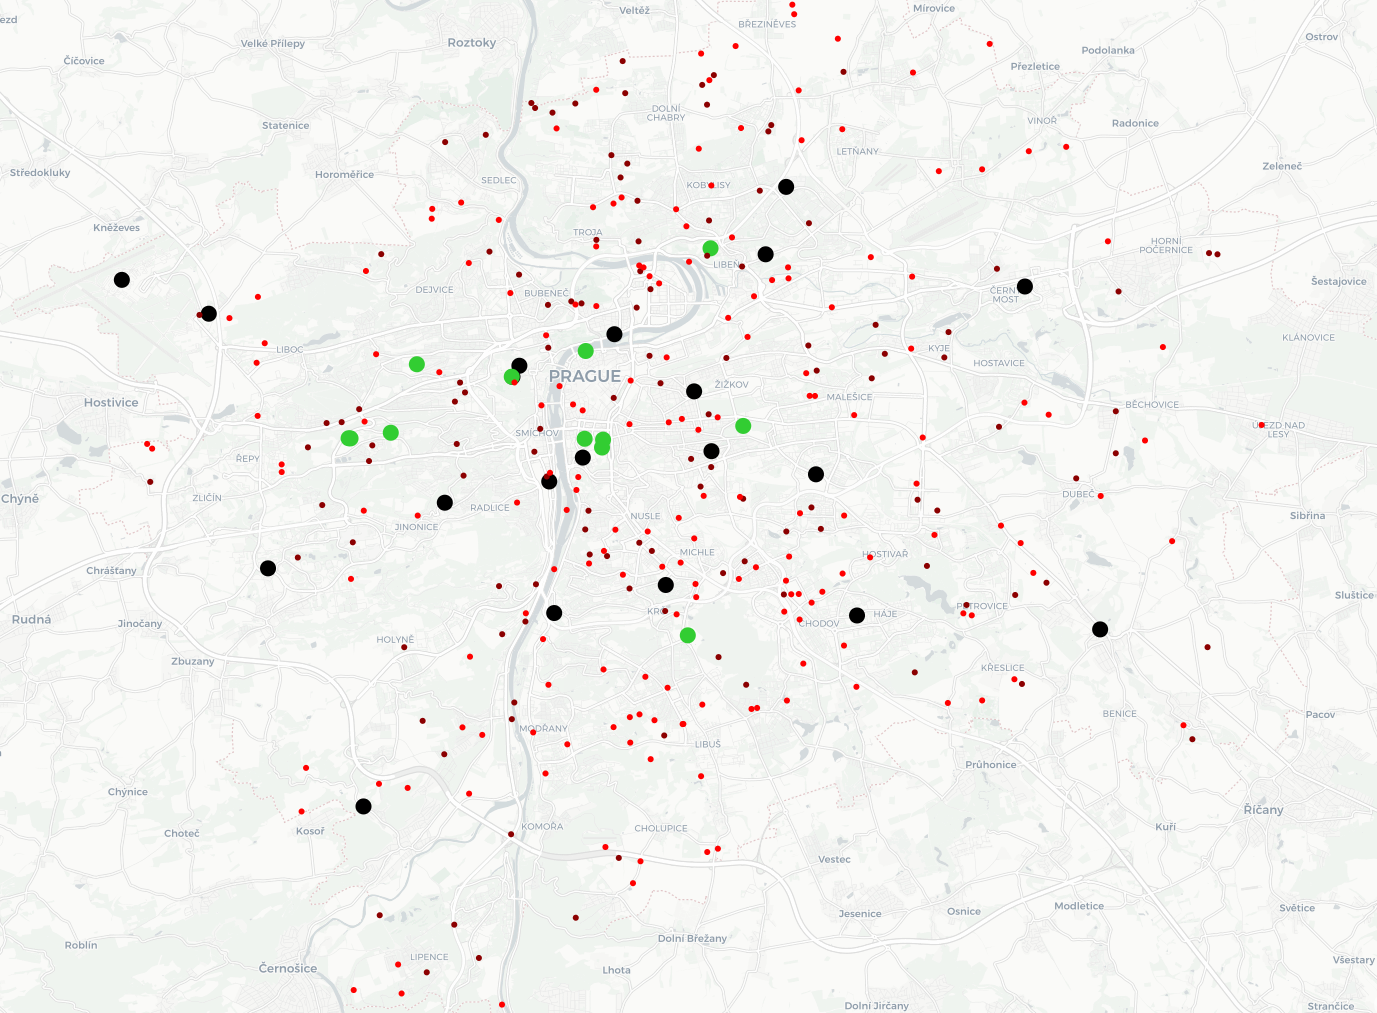
\includegraphics[width=\textwidth]{img/prague_monday_420.png}
  \centering
  \label{img:prague}
\end{figure}

Na obrázku \ref{img:prague} je znázorněno na mapě Prahy rozmístění 20 výjezdových stanic (body černé barvy), 12 nemocnic (body zelené barvy) a 300 incidentů (body červené barvy).
Tmavě červené body reprezentují incidenty, které se odehrají mezi 9 a 12 hodinou.

S výše popsanou reprezentací pohotovostní služby a sady incidentů je třeba zajistit, aby simulace uměla věrohodně zjistit doby trvání příjezdů.
Připomeňme si, že simulaci používáme právě z toho důvodu, aby počet úspěšně odbavených incidentů plánem byl co nejvěrohodnější.
Věrohodnost zajistíme použitím Google API pro zjišťování těchto dob příjezdu. Konkrétně pomocí Distance Matrix API a Routes API.

V průběhu simulace je potřeba především znát následující doby příjezdů:
\begin{enumerate}
  \item z výjezdové stanice na incident,
  \item z incidentu do nemocnice,
  \item z nemocnice zpět na výjezdovou stanici.
\end{enumerate}

Simulace podporuje i tzvn. \textit{reroute}, tedy jak se záchranný tým vrací po odbavení incidentu zpět na výjezdovou stanici,
tak je povoleno, aby mohlo z aktuální lokace vyrazit na odbavování incidentu, aniž by se musela na výjezdovou stanici vrátit.

Doby příjezdů mezi výjezdovými stanicemi, incidenty a nemocnicemi si můžeme předpočítat, ale \textit{reroute} předpočítat nelze.
Můžeme si alespoň v průběhu simulování všechny spočítané doby příjezdů mezi lokacemi udržovat s přesností na desítky metrů,
aby se v budoucnu nemuselo volat Google API, což je samozřejmě pomalá operace, trvající desítky až stovky milisekund. 

\section{Aplikace naivního řešení}

První metodu, kterou aplikujeme na namodelovanou záchrannou službu a incidenty podle předchozí kapitoly je naivní řešení.

\section{Aplikace prohledávání plánů optimálními \linebreak tahy}

V této kapitole aplikujeme algoritmus prohledávání plánů optimálními tahy \ref{alg:rekProhPlanu}.
Konkrétně použijeme jeho upravenou verzi, kde strom tahů budeme prohledávat vždy od prázdného plánu, a na každé hladině rekurze zvolíme pouze jeden náhodný optimální tah.
Oproti postupnému prohledávání všech tahů na každé úrovni má výhodu ve vyzkoušení více odlišných konfigurací a nalezené optimální plány v ceně budou s menší pravděpodobností sdílet
podobně naalokované týmy, vozidla a směny, což povede k diversifikovanějšímu prohledání množiny povolených plánů.

\begin{table}[h!]
\centering
\begin{tabular}{|c|c|c|}
\hline
\textbf{Čas běhu v minutách} & \textbf{Cena plánu} & \textbf{Odbavené incidenty} \\
\hline
7:11 & 2455260 & 292 \\
\hline
10:53 & 2469661 & 296 \\
\hline
13:38 & 2433659 & 294 \\
\hline
16:28 & 2347256 & 294 \\
\hline
19:23 & 2376058 & 293 \\
\hline
22:06 & 2340053 & 290 \\
\hline
25:14 & 2433661 & 292 \\
\hline
28:13 & 2368858 & 293 \\
\hline
30:46 & 2404856 & 294 \\
\hline
33:08 & 2448061 & 291 \\
\hline
\end{tabular}
\caption{Spuštění prohledávání optimálními tahy na modelu Prahy.}
\label{table:optimalMovesTabulka}
\end{table}

Po spuštění metody na modelu Prahy po dobu kolem 30 minut metoda celkem navštívila 10 plánů optimálních v ceně.
Nalezený optimální plán odbavuje 296 incidentů a stojí 2469661 (viz tabulka \ref{table:optimalMovesTabulka}).
Dále má naalokovaných 100 týmů a 61 záchranných vozidel.

První plán trvá nalézt nejdéle, něco přes 7 minut. Důvodem je, že \textit{cache} dob příjezdů obsahuje pouze předpočítané hodnoty a musí se vykonávat větší množství
dotazů na Google API.
Při prohledávání dalších plánů už se dotazuje na Google API mnohem méně často.
Pro zajímavost, celkový počet dotazů na dobu trvání příjezdu je 133189050, kde pro 133179688 případu, tedy $99.99\%$, byla doba příjezdu předpočítaná a vrácena z \textit{cache}.
Podobně se \textit{cache} chová i u ostatních metod.

\section{Aplikace lokálního prohledávání}

V této kapitole aplikujeme na model Prahy lokální prohledávání (viz kapitola \ref{kap:localSearch}).
Metodu použijeme přesně jak je popsaná algoritmem \ref{alg:hillclimb}.
Prohledávání začneme z prázdného plánu a jako účelovou funkci použijeme váženou sumu ceny plánu a počtu odbavených incidentů, s parametrem $\alpha = 0.99$ (viz definice \ref{df:vazenaSumaUcelF}),
abychom upřednostňovali plány s vyšším počtem odbavených incidentů.
Jakou přesně účelovou funkci si zvolíme uvážíme podle toho, co pro nás konkrétně znamená optimální plán.
My budeme chtít zkoumat především plány odbavující co nejvíce incidentů a až poté minimalizovat cenu.

Potřebujeme ještě nadefinovat jak budou vypadat sousedi nějakého plánu.
Ty standardně nadefinujeme implicitně pomocí tahů a vyžadujeme, aby splňovali alespoň nutné podmínky.
Takové tahy můžeme vybrat různě, my si vybereme tahy uvedené jako příklad tahů, které nutné podmínky splňují (viz příklad \ref{pr:sousedi}).

Záměrně alokování týmu a vozidla zvolíme jako jeden tah a nikoliv jako dva samostatné tahy. Vyhneme se tak situaci, kdy by se lokální prohledávání zastavilo v lokálním optimu, 
kde už nelze odbavit žádný incident naalokování týmu a vozidla odděleně, ale pouze zároveň. Takové lokální optimum by pak bylo suboptimální, protože by odbavovalo méně incidentů, než by mohlo být možné.
Takto definované sousedství budeme používat i u dalších metod.

\begin{figure}[H]
  \caption{Nalezené plány metodou lokálního prohledávání plánů.}
  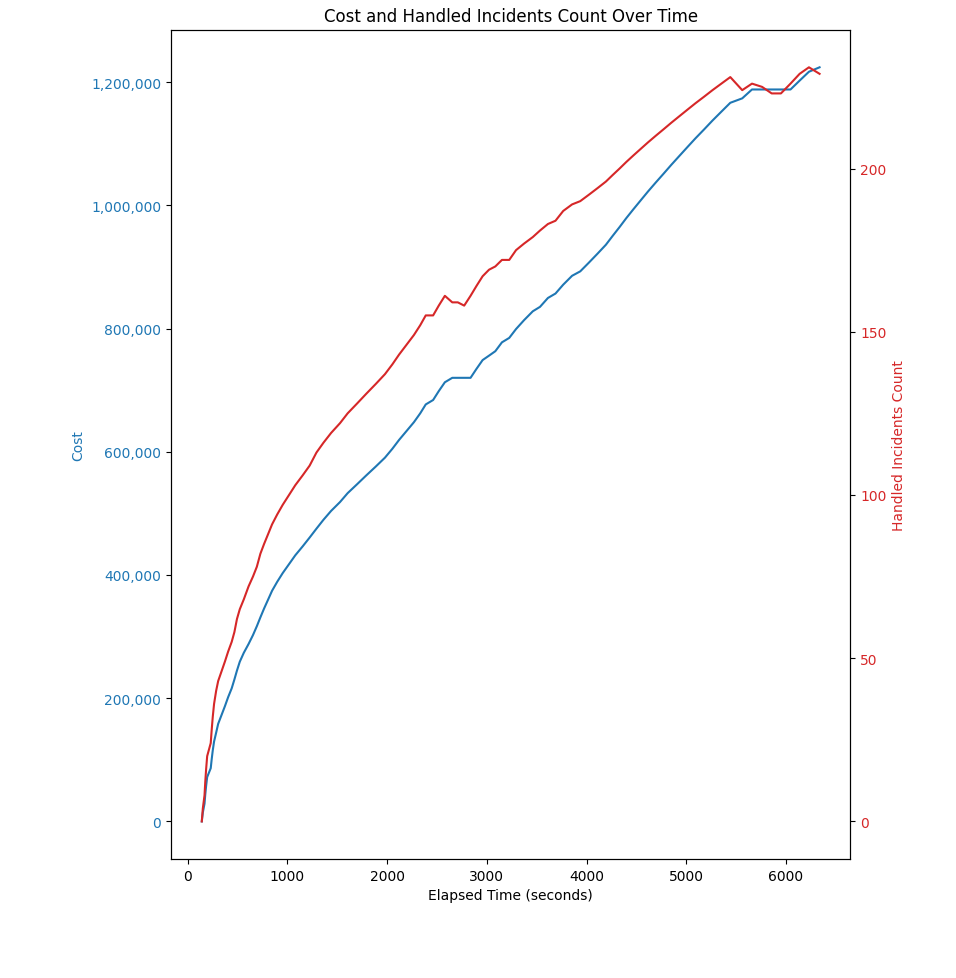
\includegraphics[width=\textwidth]{img/plots/localSearch_empty.png}
  \centering
  \label{img:localSearchRes}
\end{figure}

V grafu \ref{img:localSearchRes} vidíme jak se aktuální plán mění v čase.
Lokální prohledávání bylo spuštěné po dobu 50 minut, a pak bylo přeřušeno. 
Nejlepší nalezený plán po hodině a půl úspěšně odbaví 229 incidentů z 300 incidentů a stojí 1224080.
To je v porovnání s předchozí metodou, která za pouhých 7 minut nalezla plán odbavující 295 incidentů nedostačující výsledek.
I když by se podle růstu křivky dalo usoudit, že by metoda lokálního prohledávání také byla schopná nalézt dost dobrý plán, trvalo by to příliš dlouho.

Lokální prohledávání celkem navštívilo 29248 plánů. To je až 7 krát tolik, kolik plánů navštívila metoda prohledávání optimálními tahy.
Lokální prohledávání tedy není vhodné na budování optimálního plánu z prázdného plánu, protože zbytečně navštíví velké množství plánů a trvá tak zbytečně dlouho.

Můžeme si polepšit, sice že začneme prohledávát ne z prázdného plánu, ale z plánu zvoleného nějak chytře. Z plánu, který už je skoro optimální a lokální prohledávání
už jej jenom doladí.

Jednou z možností jak takový startovní plán zvolit je použít první nalezený optimální plán v ceně předchozí metodou a na něj spustit lokální prohledávání.

\begin{figure}[H]
  \caption{Nalezené plány metodou lokálního prohledávání plánů z plánu optimálního v ceně.}
  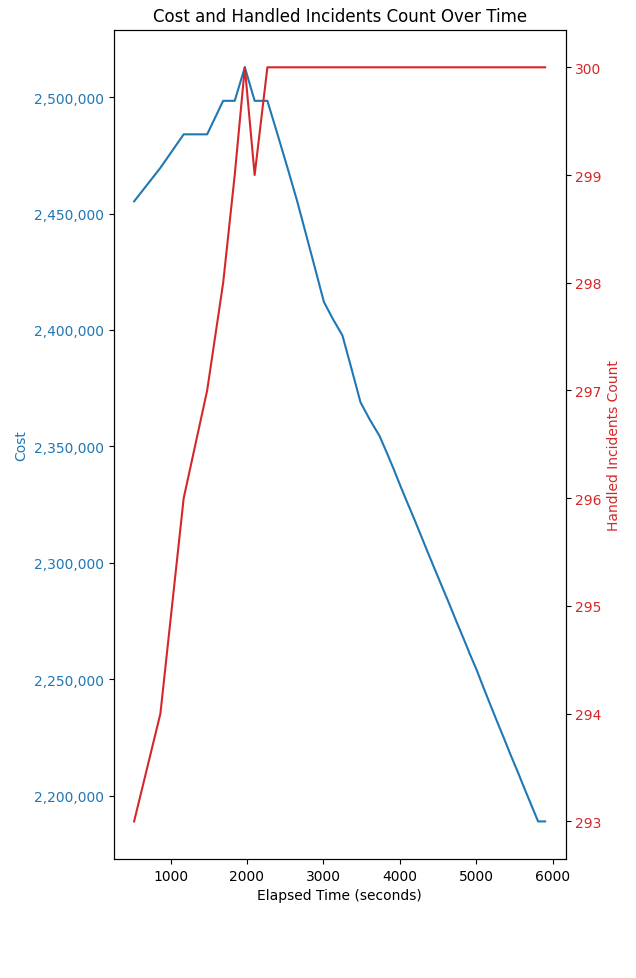
\includegraphics[width=\textwidth]{img/plots/localSearch_fromOptimal.png}
  \centering
  \label{img:hybrid}
\end{figure}

Na obrázku \ref{img:hybrid} vidíme graf, kde lokální prohledávání začíná ne z prázdného plánu, ale z plánu optimálního v ceně.
Můžeme vidět, že lokální prohledávání upravuje plán tak, že postupně odbavuje více incidentů, až nakonec všech 300. Poté už jen postupně snižuje cenu plánu.
Po zhruba 30 minutách nalezne plán odbavující všechny incidenty a do hodiny a půl lokální prohledávání stagnuje a nalezne lokální optimum.
Optimální nalezený plán odbavuje všech 300 incidentů, stojí 2188863 a má naalokovaných pouze 88 týmů a 63 vozidel.

\section{Aplikace tabu prohledávání}

V této kapitole aplikujeme na model Prahy tabu prohledávání (viz kapitola \ref{kap:tabuSearch}).
Tabu prohledávání je v podstatě lokální prohledávání s pamětí, podle které umí sofistikovaněji vybrat sousední plán,
pokud se ocitne v lokálním optimu.

\begin{figure}[H]
  \caption{Nalezené plány tabu metodou z plánu optimálního v ceně.}
  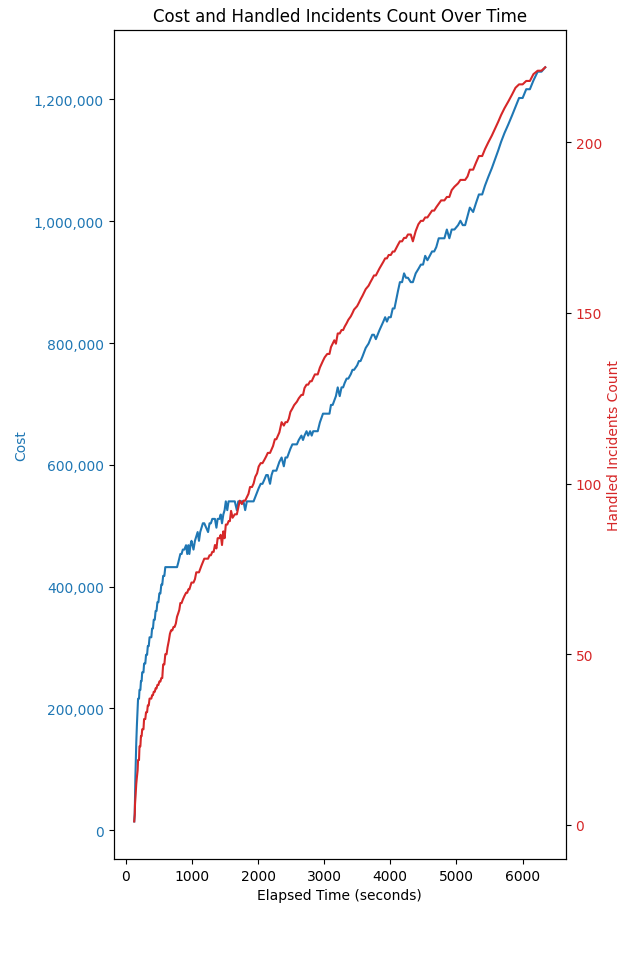
\includegraphics[width=\textwidth]{img/plots/tabuSearch_empty.png}
  \centering
  \label{img:empty_tabu}
\end{figure}

Z toho důvodu bude podobně jako u lokálního prohledávání (viz obrázek \ref{img:empty_tabu}) trvat příliš dlouho, než nalezne nějaký dost dobrý plán.
Obdobně jako u lokálního prohledávání nemá smysl pouštět tabu prohledávání z prázdného plánu.

\begin{figure}[H]
  \caption{Nalezené plány tabu metodou z plánu optimálního v ceně.}
  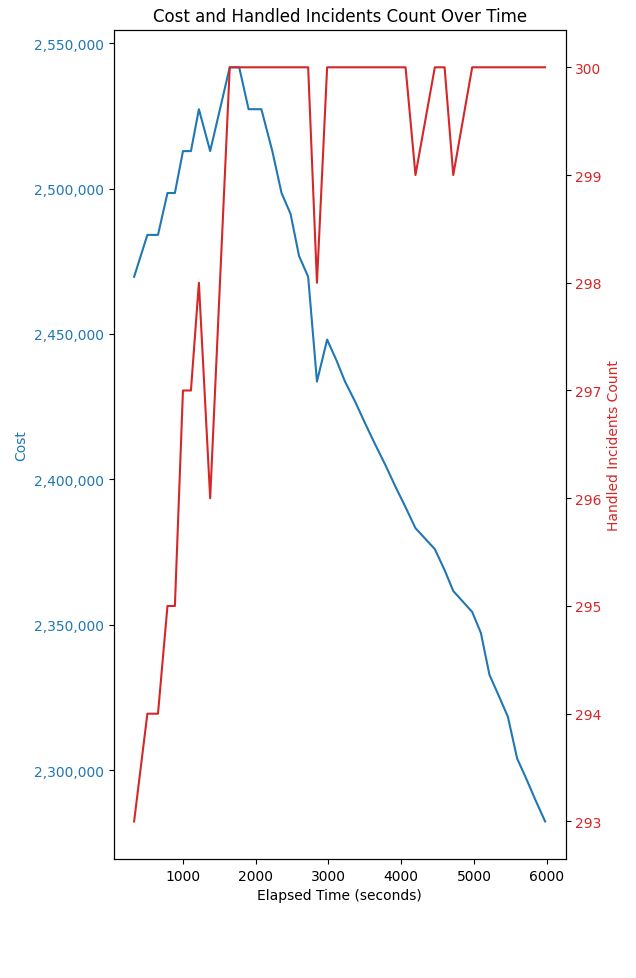
\includegraphics[width=\textwidth]{img/plots/tabuSearch_fromOptimal.png}
  \centering
  \label{img:hybrid_tabu}
\end{figure}

Na obrázku \ref{img:hybrid_tabu} vidíme doposud nejlepší plány nalezené tabu metodou v čase z plánu optimálního v ceně.
Nalézt plán odbavující všech 300 incidentů trvá kolem 40 minut, což je o 10 minut déle, než trvalo lokálnímu prohledávání. 
To je pochopitelné, protože při navštívení každého souseda, kterých bude obdobně jako u lokálního prohledávání, se musí kontrolovat,
zda není obsažen v tabu. Proto vyhodnocení souseda bude trvat o něco déle, což se při tak velkém množství navštívených plánů poměrně rychle nasčítá.

Tabu prohledávání bylo puštěno něco kolem hodiny a půl, a obdobně jako u lokálního prohledávání, s roustoucí délkou běhu programu se i snižuje cena plánu.
Výhoda tabu prohledávání je hlavně v schopnosti nezůstat v lokálním optimu a umět robustněji prohledávat prostor konfigurací.
Tato výhoda v našem případě ale není využita, protože tabu prohledávání ani za hodinu běhu na lokální optimum nenarazilo.
Spíše naopak, prohledávání tabu je nevýhodou, a lokální prohledávání je v tomto případě lepší volbou.

\section{Aplikace simulovaného žíhání}

V této kapitole aplikujeme na model Prahy simulované žíhání (viz kapitola \ref{kap:tabuSearch}).
Simulovanému žíhání je potřeba nastavit následující hyperparametry:
\begin{enumerate}
  \item počáteční teplota,
  \item koncová teplota,
  \item chladící rozvrh,
  \item počet iterací v rámci stejné teploty.
\end{enumerate}

Počáteční teplota je vhodné nastavit tak, aby pravděpodobnost přijetí horší konfigurace byla ze začátku kolem 0.8--0.9 procent \cite{sa_theory}.
Vzhledem k tomu, že používáme váženou sumu účelových funkcí, tak se výsledná hodnota účelové funkce pohybuje mezi 0 a 1.
Tím pádem rozdíl se pohybuje mezi -1 a 1.
Pokud je $\Delta$ záporná, tak je sousední plán vždy navštíven, protože je
jeho hodnota při účelové funkci vyšší. Zajímá nás tedy pouze případ, kdy je $\Delta$ nekladná.

Připomeňme si jak vypadá akceptační kritérium:
\begin{align*}\label{df:metropolis}
  \exp\left(-\frac{\Delta q}{t}\right).
\end{align*}

Počáteční teplota splňující takový požadavek činí například 5 stupňů, jak můžeme vidět na obrázku \ref{img:metropolis_5},
kde na ose x je hodnota delta, a na ose y pravděpodobnost přijetí sousedního plánu metropolisním kritériem, který se od aktuálního liší o danou deltu.

\begin{figure}[H]
  \centering
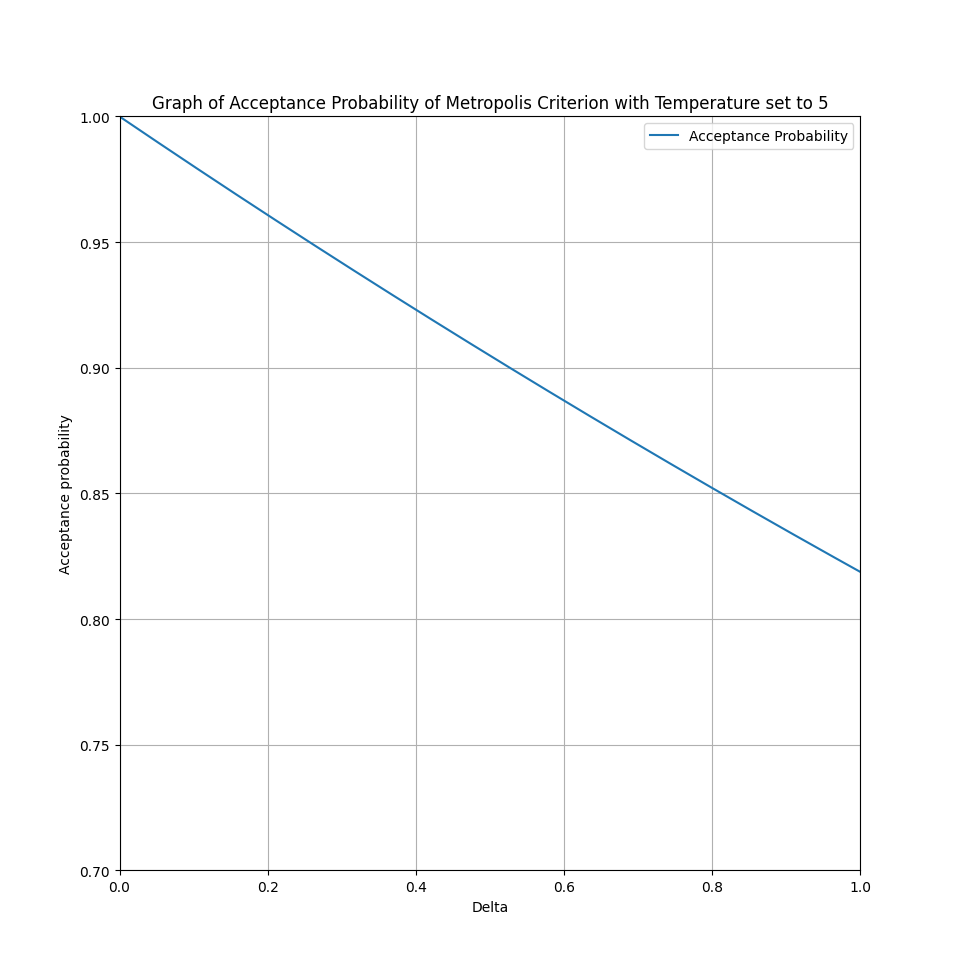
\includegraphics[width=0.5\textwidth,height=0.5\textwidth]{img/metropolis_5.png}
  \caption{Metropolis kritérium pro teplotu 5 stupňů.}
  \label{img:metropolis_5}
\end{figure}

Finální teplota se často volí velmi blízko nule, aby bylo možné dostatečně důkladně prohledat konfigurace lokálně, podobně jak dělá například lokální prohledávání \cite{sa_theory}.
Zatím vyberme finální teplotu jako $10^{-6}$.

Vybrat ochlazovací rozvrh lze různě, nejčastěji používané jsou \cite{sa_theory}:
\begin{enumerate}
  \item Lineární chladící rozvrh, kde se teplota aktualizuje následovně:
    \begin{align*}
      t_{k+1} = t_k - k \cdot \Delta t_k,
    \end{align*}
    kde $t_k$ je aktuální teplota, $t_{k+1}$ je nová teplota a $\Delta t_k$ je hyperpametr, o kolik teplotu snižovat.
    Je velmi jednoduchý na implementaci, ale není tak dobrý jako ostatní ochlazující rozvrhy \cite{sa_schedules}.

  \item Logaritmický ochlazující rozvrh:
    \begin{align*}
      t_{k+1} = t_{k} / \log(1 + k).
    \end{align*}
    Logaritmický ochlazující rozvrh má dobré teoretické vlastnosti, ovšem pro praktické použití je příliš pomalý \cite{sa_schedules}.

  \item Exponenciální ochlazující rozvrh:
    \begin{align*}
      t_{k+1} = t_k \cdot \alpha,
    \end{align*}
    kde $\alpha$ se často volí mezi 0.8 a 0.99 \cite{sa_theory}.
    Podobně jako předchozí ochlazující rozvrhy je velmi jednoduchý na implementaci, a často bývá dobrou první volbou, protože umí najít dobrý balanc mezi explorační fází,
    kdy je teplota vyšší a mezi ladící fází, kdy je teplota nižší \cite{sa_theory}.

  \item Adaptující se ochlazující rozvrh. Algoritmus si sám v průběhu nastavuje teplotu podle chování a doposud nalezených konfigurací.
    Náročnější na implementaci než předchozí ochlazující rozvrhy. Hodí se uvažovat o jeho použití především, pokud jednodušší ochlazující rozvrhy nalézají pouze suboptimální řešení.
\end{enumerate}

My si jako ochlazovací rozvrh zvolíme exponenciální ochlazovací rozvrh, především pro jeho jedhoduchou implementaci a pěkné vlastnosti.
Parametr $\alpha$ určující rychlost snižování teploty zatím zvolíme jako $0.99$.

Nelze obecně říct, kolik iterací $M_k$ provést v rámci stejné teploty. Menší počet iterací může vést k předčasné kovergenci, ale na druhou stranu je výpočet méně náročný. \cite{sa_theory}. 
Zvolme zatím pouze jednu iteraci, čili $M_k = 1$.
Je vhodné balancovat $M_k$ spolu s $\alpha$, pro zajištění rozumné výpočetní náročnosti.
Samozřejmě, že ideální je použít $\alpha$ rovno $O.99$ a $M_k$ velmi vysoké, například v rámci stovek až tisíců, 
ovšem simulované žíhání s takto zvolenými parametry je velmi výpočetně náročné a běh by trval příliš dlouho.

Jako první spustíme simulované žíhání z prázdného plánu.

\begin{figure}[H]
  \caption{Simulované žíhání z prázdného plánu.}
  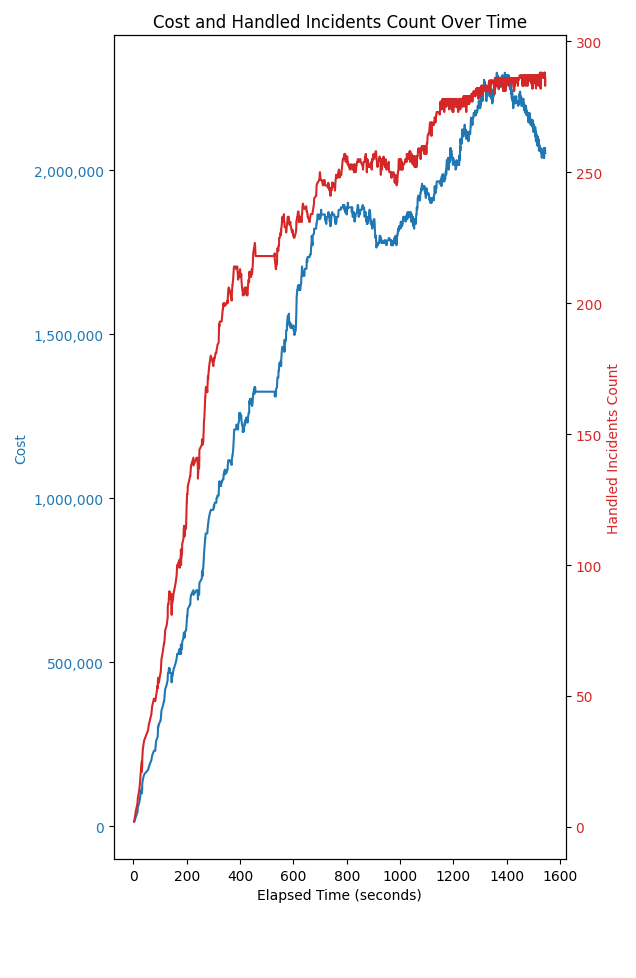
\includegraphics[width=\textwidth]{img/plots/sa_empty.png}
  \centering
  \label{img:sa_empty}
\end{figure}

V grafu \ref{img:sa_empty} vidíme, jaké plány simulované žíhání
s počáteční teplotou 5 stupňů, finální teplotou $10^{-6}$, exponenciálním chladícím rozvrhem s $\alpha = 0.99$ a s $M_k = 1$,
v průběhu z prázdného plánu navštěvovalo.
Celkově běželo simulované žíhání 25 minut a navštívilo celkem 1779 plánů.
Nejlepší nalezený plán odbavuje 288 incidentů, stojí 2059332 a má naalokovaných 93 týmů a 132 záchranných vozidel.
V porovnání s lokálním nebo tabu prohledáváním z prázdného plánu se jedná o dramaticky lepší výsledek.

Podobně jako u předchozích metod můžeme zkusit spustit simulované žíhání z jiného než prázdného plánu.
Zkusme spustit z uniformě náhodně vygenerovaného plánu, který má naalokovaných zhruba 50\% týmů a vozidel.

\begin{figure}[H]
  \caption{Simulované žíhání z náhodného plánu.}
  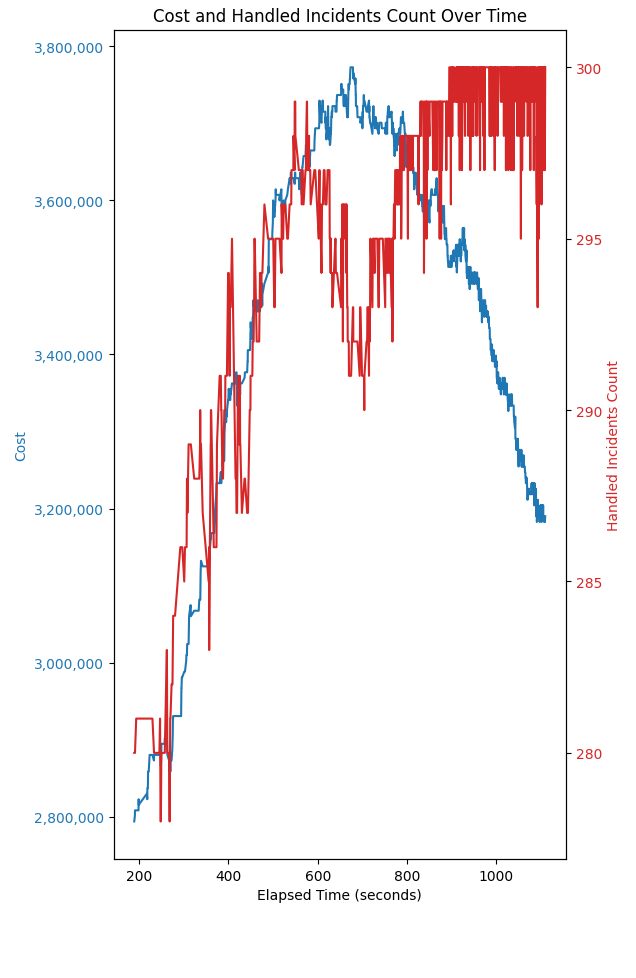
\includegraphics[width=\textwidth]{img/plots/sa_random_85.png}
  \centering
  \label{img:sa_random}
\end{figure}

V grafu \ref{img:sa_random} vidíme chování simulovaného žíhání
s počáteční teplotou 5 stupňů, finální teplotou $10^{-6}$, exponenciálním chladícím rozvrhem s $\alpha = 0.85$ a s $M_k = 10$,
Přibližně do 12 minuty (800 sekund) lze vidět explorační fázi, kdy následně už je plán pouze lokálně vylepšován. 
Spustit simulované žíhání z náhodného plánu přináší lepší výsledky než z plánu prázdného.
Nejlepší nalezený plán odbavuje všech 300 incidentů, stojí 3182531 a má naalokovaných 139 týmů a 126 vozidel.

Z grafu podle klesající ceny můžeme usoudit, že by simulované žíhání bylo schopné najít ještě lepší plán, pokud by mohlo běžet déle.
Spusťmě proto simulované žíhání znovu ze stejného náhodného plánu, tentorkát ale s jinými parametry.

\begin{figure}[H]
  \caption{Simulované žíhání z náhodného plánu.}
  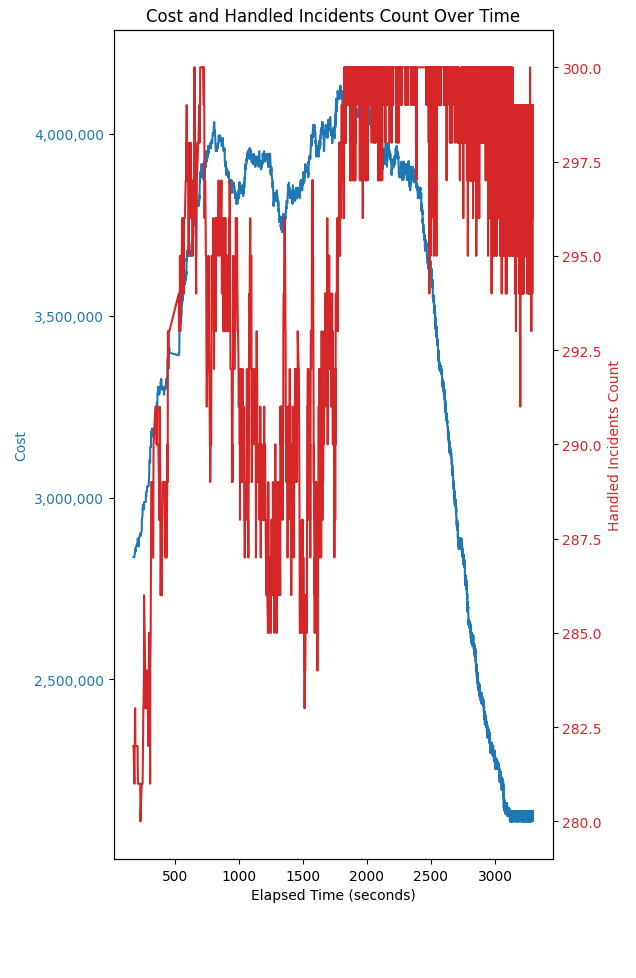
\includegraphics[width=\textwidth]{img/plots/sa_random_90.png}
  \centering
  \label{img:sa_random}
\end{figure}

V grafu \ref{img:sa_random} vidíme chování simulovaného žíhání
s počáteční teplotou 3 stupňů, finální teplotou $10^{-8}$, exponenciálním chladícím rozvrhem s $\alpha = 0.90$ a s $M_k = 30$,
Finální teplota je snížena, aby se prodloužila ladící fáze.
Zároveň je snížena rychlost klesání teploty a zvýšen počet iterací v rámci stejné teploty, takže sice bude výpočet trvat déle, ale zato by měl být nalezený optimální plán lepší.
Skutečně, optimální nalezený plán odbavuje všech 300 incidentů, stojí 2124103 a má naalokovaných 94 týmů a 104 vozidel.

Zkusme ještě spustit simulované žíhání z plánu optimálního v ceně, podobně jako u lokálního a tabu prohledávání.

\begin{figure}[H]
  \caption{Simulované žíhání z plánu optimálního v ceně.}
  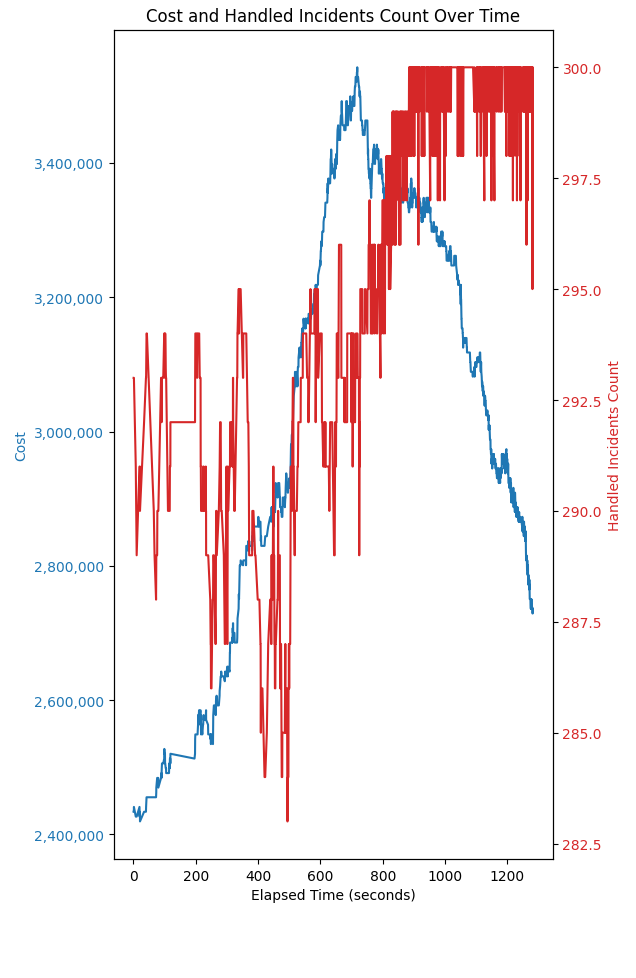
\includegraphics[width=\textwidth]{img/plots/sa_optimal.png}
  \centering
  \label{img:sa_optimal}
\end{figure}

V grafu \ref{img:sa_optimal} vidíme průběh výpočtu.
Podobně jako v případě procházení z náhodného plánu jsou při vyšší teplotě navštěvovány horší plány v rámci explorace a od přibližně 
10 minuty (700 sekund) se postupně přechází do ladící fáze, která se chová podobně jako lokální prohledávání.
Program celkově běžel něco pod 30 minut i spolu s nalezením plánu optimálního v ceně.
Nejlepší nalezený plán odbavuje 300 incidentů, stojí 2736133 a má naalokovaných 108 týmu a 133 vozidel.


\chapter{Implementace}

\section{Implementace simulace}

\section{Návrh programu}

\section{Uživatelská dokumentace}



\chapter*{Závěr}
\addcontentsline{toc}{chapter}{Závěr}

Tato práce se zabývá problémem nalezení optimálního plánu pohotovostní služby. 
V první kapitole jsme problém zformalizovali a důkladně zanalyzovali, abychom zvolili vhodné metody řešení.
Ukázalo se, že nejvhodnější je problém modelovat jako optimalizační úlohu s jednou účelovou funkcí.
Účelová funkce je vhodným složením ceny plánu a počtu úspěšně odbavených incidentů.
Abychom věrohodně zjistili počet úspěšně odbavených incidentů, spustili jsme diskrétní simulaci, která pro danou sadu incidentů napodobuje chování plánu v průběhu jednoho dne.
Použití simulace omezilo možné techniky, které se běžně používají pro řešení těžkých optimalizačních problému, jako například lineární programování.
Na druhou stranu, umožňuje věrohodně získat počet úspěšně odbavených incidentů, stejně jako by plán již skutečně odbavoval incidenty v terénu.
 
V druhé kapitole jsme diskutovali několik různých metod, od využití dynamického programování, až po použití metaheuristických přístupů.
Nalezli jsme rekurzivní vztah mezi plány odbavující o jedna méně incidentů
a využili jej pro řešení úlohy pomocí dynamického programování. Přestože výpočetní složitost je exponenciální vůči počtu incidentů, 
jedná se o dramatické zlepšení oproti naivnímu řešení, které jenom náhodně vytváří plány.

Ve třetí kapitole jsme nalezené metody aplikovali na konkrétní pohotovostní službu, a to sice na pohotovostní službu hlavního města Prahy.
Synteticky jsme vygenerovali sadu incidentů, která vhodně reprezentuje možnou skutečnou situaci.
Na základě volně dostupných dat pražské pohotovostní služby představuje, jak by se mohly incidenty v průběhu dne skutečně odehrát.

Při aplikaci metod jsme zjistili, že některé metody jsou vhodnější než jiné. Například se ukázalo, že nemá smysl používat tabu prohledávání, jelikož je obtížné nalézt i jedno lokální optimum.
Na druhou stranu, kombinace lokálního prohledávání nebo simulovaného žíhání spolu s dynamickým programováním se ukázaly jako nejlepší metody pro praktické využití.
Nalezené plány uměly úspěšně odbavit všechny incidenty jen s polovinou vozidel a do stovky týmů záchranářů.
Nalezené plány jsou kvalitní, a jistě by se uplatnily pro praktické využití.

Přestože umíme nalézt velmi kvalitní plány pohotovostní služby na dané sadě incidentů, lze práci do budoucna rozšířit hned o několik věcí.
Především by bylo zajímavé více prozkoumat, jak vypadají optimální plány, které by odbavovaly jen o něco méně incidentů, ale byly by výrazně levnější.
Takové plány by se daly hledat pomocí vhodně zvolené účelové funkce, která by poskytovala dobře nastavený kompromis mezi cenou a počtem odbavených incidentů. 

Dalším zajímavým rozšířením by bylo přidat incidentům typ, který by určoval, jaká záchranná vozidla a týmy by mohly incident odbavit.
Jednotlivé týmy nebo vozidla by byly různě drahé, právě podle toho, jaké typy incidentů by mohly odbavovat. 
Implementace takového rozšíření vyžaduje pouze úpravu simulace a přidání nových tahů u metod, které využívají sousedství.

V neposlední řadě by bylo zajímavé zkoumat, jak se nalezené optimální plány chovájí v krajních případech, kdy se například najednou stane velké množství incidentů
na jedné lokalitě, nebo na velmi odlehlé lokalitě, případně i ve stejný čas. Aby bylo možné takové plány hledat, je potřeba, aby plány uměly dobře generalizovat.
Metody by tak musely krajní případy uvažovat už v rámci hledání a předem alokovat vozidla a týmy, i když by většinu času nebyly potřeba.
To nás vede na další rozšíření, kdy by bylo dovoleno, aby týmy naalokované na jedné výjezdové stanici mohly pomáhat v krajních případech týmům na jiných stanicích.
Tomuto mechanismu se říká \textit{dynamic dispatch} a v krajních případech by se mohlo jednat o nejefektivnější způsob, jak zdroje rozmisťovat.



%%% Seznam použité literatury
%%% Seznam použité literatury (bibliografie)
%%%
%%% Pro vytváření bibliografie používáme biblatex. Ten zpracovává
%%% citace v textu (např. makro \cite{...}) a vyhledává k nim literaturu
%%% v souboru literatura.bib.
%%%
%%% Podívejte se na nastavení biblatexu v souboru thesis.tex.

%%% Vytvoření seznamu literatury. Pozor, pokud jste necitovali ani jednu
%%% položku, seznam se automaticky vynechá.

% Dovolíme položkám trochu vyčuhovat přes pravý okraj.
\def\bibfont{\hfuzz=2pt}

\printbibliography[heading=bibintoc,title=Literatura]

%%% Kdybyste chtěli bibliografii vytvářet ručně (bez biblatexu), lze to udělat
%%% následovně. V takovém případě se řiďte normou ISO 690 a zvyklostmi v oboru.

% \begin{thebibliography}{99}
%
% \bibitem{lamport94}
%   {\sc Lamport,} Leslie.
%   \emph{\LaTeX: A Document Preparation System}.
%   2. vydání.
%   Massachusetts: Addison Wesley, 1994.
%   ISBN 0-201-52983-1.
%
% \end{thebibliography}


%%% Obrázky v práci
%%% (pokud jich je malé množství, obvykle není třeba seznam uvádět)
\listoffigures

%%% Tabulky v práci (opět nemusí být nutné uvádět)
%%% U matematických prací může být lepší přemístit seznam tabulek na začátek práce.
\listoftables

%%% Použité zkratky v práci (opět nemusí být nutné uvádět)
%%% U matematických prací může být lepší přemístit seznam zkratek na začátek práce.
\chapwithtoc{Seznam použitých zkratek}

%%% Součástí doktorských prací musí být seznam vlastních publikací
\ifx\ThesisType\TypePhD
\chapwithtoc{Seznam publikací}
\fi

%%% Přílohy k práci, existují-li. Každá příloha musí být alespoň jednou
%%% odkazována z vlastního textu práce. Přílohy se číslují.
%%%
%%% Do tištěné verze se spíše hodí přílohy, které lze číst a prohlížet (dodatečné
%%% tabulky a grafy, různé textové doplňky, ukázky výstupů z počítačových programů,
%%% apod.). Do elektronické verze se hodí přílohy, které budou spíše používány
%%% v elektronické podobě než čteny (zdrojové kódy programů, datové soubory,
%%% interaktivní grafy apod.). Elektronické přílohy se nahrávají do SISu.
%%% Povolené formáty souborů specifikuje opatření rektora č. 72/2017.
%%% Výjimky schvaluje fakultní koordinátor pro zavěrečné práce.
\appendix
\chapter{Přílohy}

\section{První příloha}

\end{document}
